%% Include all the following packages. Feel free to add other packages if needed.

\documentclass[12pt]{thesis} 
\usepackage{amsmath,amssymb,amsthm,amsfonts}
\usepackage[]{mcode}
\usepackage[draft]{graphicx}
\graphicspath{ {./figures/} }
\usepackage{array,multirow,graphicx}
\usepackage{booktabs, multirow, array, makecell, caption}
\usepackage[flushleft]{threeparttable}
\usepackage{pbox}
\usepackage{enumerate}
\usepackage[stable]{footmisc}
\usepackage{epstopdf}
\usepackage{amsmath}
\DeclareGraphicsExtensions{.eps}
\graphicspath{{./figures/}} % I added this so the figures are all in one folder
\usepackage{array}
\usepackage{pgfgantt}
\usepackage{xcolor}
%\usepackage{chemformula}
\usepackage{xfrac}
\usepackage{float}
\usepackage{tabularx}
\usepackage{hyphenat}
\usepackage{makecell}%To keep spacing of text in tables
\usepackage{bbm}
%\usepackage{setspace}
\usepackage{footmisc}
\renewcommand\footnotelayout{\fontsize{11}{7}\selectfont  }
\usepackage{rotating}


\captionsetup{labelfont={bf}}
\captionsetup[table]{font={stretch=1}}    
\captionsetup[figure]{font={stretch=1}}   


\renewcommand\bibname{REFERENCES}

\captionsetup{justification=raggedright,singlelinecheck=false}


\DeclareCaptionLabelSeparator{none}{ }
\captionsetup{labelsep=none}


%%%%%%%%%%%%% MACROS
\newcommand{\calA}{\mathcal{A}}%
\newcommand{\calB}{\mathcal{B}}%
\newcommand{\calC}{\mathcal{C}}%
\newcommand{\calD}{\mathcal{D}}%
\newcommand{\calE}{\mathcal{E}}%
\newcommand{\calF}{\mathcal{F}}%
\newcommand{\calH}{\mathcal{H}}%
\newcommand{\calI}{\mathcal{I}}%
\newcommand{\calJ}{\mathcal{J}}%
\newcommand{\calK}{\mathcal{K}}%
\newcommand{\calL}{\mathcal{L}}%
\newcommand{\calM}{\mathcal{M}}%
\newcommand{\calN}{\mathcal{N}}%
\newcommand{\calP}{\mathcal{P}}%cc
\newcommand{\calQ}{\mathcal{Q}}%
\newcommand{\calR}{\mathcal{R}}%
\newcommand{\calS}{\mathcal{S}}%
\newcommand{\calV}{\mathcal{V}}%
\newcommand{\calW}{\mathcal{W}}%
\newcommand{\calX}{\mathcal{X}}%
\newcommand{\calT}{\mathcal{T}}%
%
%
\newcommand{\bfa}{{\bf a}}\newcommand{\bfA}{{\bf A}}%
\newcommand{\bfb}{{\bf b}}\newcommand{\bfB}{{\bf B}}%
\newcommand{\bfc}{{\bf c}}\newcommand{\bfC}{{\bf C}}%
\newcommand{\bfd}{{\bf d}}\newcommand{\bfD}{{\bf D}}%
\newcommand{\bfe}{{\bf e}}\newcommand{\bfE}{{\bf E}}%
\newcommand{\bff}{{\bf f}}\newcommand{\bfF}{{\bf F}}%
\newcommand{\bfg}{{\bf g}}\newcommand{\bfG}{{\bf G}}%
\newcommand{\bfh}{{\bf h}}\newcommand{\bfH}{{\bf H}}%
\newcommand{\bfi}{{\bf i}}\newcommand{\bfI}{{\bf I}}%
\newcommand{\bfj}{{\bf j}}\newcommand{\bfJ}{{\bf J}}%
\newcommand{\bfk}{{\bf k}}\newcommand{\bfK}{{\bf K}}%
\newcommand{\bfl}{{\bf l}}\newcommand{\bfL}{{\bf L}}%
\newcommand{\bfm}{{\bf m}}\newcommand{\bfM}{{\bf M}}%
\newcommand{\bfn}{{\bf n}}\newcommand{\bfN}{{\bf N}}%
\newcommand{\bfo}{{\bf o}}\newcommand{\bfO}{{\bf O}}%
\newcommand{\bfp}{{\bf p}}\newcommand{\bfP}{{\bf P}}%
\newcommand{\bfq}{{\bf q}}\newcommand{\bfQ}{{\bf Q}}%
\newcommand{\bfr}{{\bf r}}\newcommand{\bfR}{{\bf R}}%
\newcommand{\bfs}{{\bf s}}\newcommand{\bfS}{{\bf S}}%
\newcommand{\bft}{{\bf t}}\newcommand{\bfT}{{\bf T}}%
\newcommand{\bfu}{{\bf u}}\newcommand{\bfU}{{\bf U}}%
\newcommand{\bfv}{{\bf v}}\newcommand{\bfV}{{\bf V}}%
\newcommand{\bfw}{{\bf w}}\newcommand{\bfW}{{\bf W}}%
\newcommand{\bfx}{{\bf x}}\newcommand{\bfX}{{\bf X}}%
\newcommand{\bfy}{{\bf y}}\newcommand{\bfY}{{\bf Y}}%
\newcommand{\bfz}{{\bf z}}\newcommand{\bfZ}{{\bf Z}}%
\newcommand{\bfell}{\boldsymbol{\ell}}%
\newcommand{\bfimath}{\boldsymbol{\imath}}%
\newcommand{\bfjmath}{\boldsymbol{\jmath}}%
\newcommand{\bfwp}{\boldsymbol{\wp}}%
\newcommand{\bfalpha}{\boldsymbol{\alpha}}%
\newcommand{\bfbeta}{\boldsymbol{\beta}}%
\newcommand{\bfgamma}{\boldsymbol{\gamma}}%
\newcommand{\bfdelta}{\boldsymbol{\delta}}%
\newcommand{\bfepsilon}{\boldsymbol{\epsilon}}%
\newcommand{\bfzeta}{\boldsymbol{\zeta}}%
\newcommand{\bfeta}{\boldsymbol{\eta}}%
\newcommand{\bftheta}{\boldsymbol{\theta}}%
\newcommand{\bfiota}{\boldsymbol{\iota}}%
\newcommand{\bfkappa}{\boldsymbol{\kappa}}%
\newcommand{\bflambda}{\boldsymbol{\lambda}}%
\newcommand{\bfmu}{\boldsymbol{\mu}}%
\newcommand{\bfnu}{\boldsymbol{\nu}}%
\newcommand{\bfxi}{\boldsymbol{\xi}}%
\newcommand{\bfpi}{\boldsymbol{\pi}}%
\newcommand{\bfrho}{\boldsymbol{\rho}}%
\newcommand{\bfsigma}{\boldsymbol{\sigma}}%
\newcommand{\bftau}{\boldsymbol{\tau}}%
\newcommand{\bfupsilon}{\boldsymbol{\upsilon}}%
\newcommand{\bfphi}{\boldsymbol{\phi}}%
\newcommand{\bfchi}{\boldsymbol{\chi}}%
\newcommand{\bfpsi}{\boldsymbol{\psi}}%
\newcommand{\bfomega}{\boldsymbol{\omega}}%
\newcommand{\bfvarepsilon}{\boldsymbol{\varepsilon}}%
\newcommand{\bfvartheta}{\boldsymbol{\vartheta}}%
\newcommand{\bfvarpi}{\boldsymbol{\vaarphi}}%
\newcommand{\bfvarrho}{\boldsymbol{\varrho}}%
\newcommand{\bfvarsigma}{\boldsymbol{\varsigma}}%
\newcommand{\bfvarphi}{\boldsymbol{\varphi}}%
%
\newfont{\tenbfit}{cmmib10}%
\newfont{\svnbfit}{cmmib8}%
\newfont{\tenbfsl}{cmbxti10}% <-- for idem tensor
\newcommand{\bfGamma}{\mbox{\tenbfit\char'00\/}}%
\newcommand{\bfDelta}{\mbox{\tenbfit\char'01\/}}%
%\newcommand{\bfTheta}{\mbox{\tenbfit\char'02\/}}%
\newcommand{\bfTheta}{\boldsymbol{\Theta}}%
\newcommand{\bfLambda}{\boldsymbol{\Lambda}}%
\newcommand{\bfXi}{\mbox{\tenbfit\char'04\/}}%
\newcommand{\bfPi}{\mbox{\tenbfit\char'05\/}}%
\newcommand{\bfSigma}{\boldsymbol{\Sigma}}%
\newcommand{\bfUpsilon}{\mbox{\tenbfit\char'07\/}}%
\newcommand{\bfPhi}{\boldsymbol{\Phi}}
\newcommand{\bfPsi}{\mbox{\tenbfit\char'11\/}}%
\newcommand{\bfOmega}{\boldsymbol{\Omega}}
\newcommand{\sbfGamma}{\mbox{\svnbfit\char'00\/}}%
\newcommand{\sbfDelta}{\mbox{\svnbfit\char'01\/}}%
\newcommand{\sbfTheta}{\mbox{\svnbfit\char'02\/}}%
\newcommand{\sbfLambda}{\mbox{\svnbfit\char'03\/}}%
\newcommand{\sbfXi}{\mbox{\svnbfit\char'04\/}}%
\newcommand{\sbfPi}{\mbox{\svnbfit\char'05\/}}%
\newcommand{\sbfSigma}{\mbox{\svnbfit\char'06\/}}%
\newcommand{\sbfUpsilon}{\mbox{\svnbfit\char'07\/}}%
\newcommand{\sbfPhi}{\mbox{\svnbfit\char'10\/}}%
\newcommand{\sbfPsi}{\mbox{\svnbfit\char'11\/}}%
\newcommand{\sbfOmega}{\mbox{\svnbfit\char'12\/}}%
%
\newfont{\mmit}{cmmi10}% scaled 1200
\newfont{\smit}{cmmi9}%  scaled 1200
\newfont{\bfMit}{cmmi5}%  scaled 1200
%
\newcommand{\iGamma}{\mbox{\mmit\char'00\/}}%
\newcommand{\iDelta}{\mbox{\mmit\char'01\/}}%
\newcommand{\iTheta}{\mbox{\mmit\char'02\/}}%
\newcommand{\iLambda}{\mbox{\mmit\char'03\/}}%
\newcommand{\iXi}{\mbox{\mmit\char'04\/}}%
\newcommand{\iPi}{\mbox{\mmit\char'05\/}}%
\newcommand{\iSigma}{\mbox{\mmit\char'06\/}}%
\newcommand{\iUpsilon}{\mbox{\mmit\char'07\/}}%
\newcommand{\iPhi}{\mbox{\mmit\char'10\/}}%
\newcommand{\iPsi}{\mbox{\mmit\char'11\/}}%
\newcommand{\iOmega}{\mbox{\mmit\char'12\/}}%
%
\newcommand{\siGamma}{\mbox{\smit\char'00\/}}%
\newcommand{\siDelta}{\mbox{\smit\char'01\/}}%
\newcommand{\siTheta}{\mbox{\smit\char'02\/}}%
\newcommand{\siLambda}{\mbox{\smit\char'03\/}}%
\newcommand{\siXi}{\mbox{\smit\char'04\/}}%
\newcommand{\siPi}{\mbox{\smit\char'05\/}}%
\newcommand{\siSigma}{\mbox{\smit\char'06\/}}%
\newcommand{\siUpsilon}{\mbox{\smit\char'07\/}}%
\newcommand{\siPhi}{\mbox{\smit\char'10\/}}%
\newcommand{\siPsi}{\mbox{\smit\char'11\/}}%
\newcommand{\siOmega}{\mbox{\smit\char'12\/}}%
%
\newcommand{\ssiGamma}{\mbox{\bfMit\char'00\/}}%
\newcommand{\ssiDelta}{\mbox{\bfMit\char'01\/}}%
\newcommand{\ssiTheta}{\mbox{\bfMit\char'02\/}}%
\newcommand{\ssiLambda}{\mbox{\bfMit\char'03\/}}%
\newcommand{\ssiXi}{\mbox{\bfMit\char'04\/}}%
\newcommand{\ssiPi}{\mbox{\bfMit\char'05\/}}%
\newcommand{\ssiSigma}{\mbox{\bfMit\char'06\/}}%
\newcommand{\ssiUpsilon}{\mbox{\bfMit\char'07\/}}%
\newcommand{\ssiPhi}{\mbox{\bfMit\char'10\/}}%
\newcommand{\ssiPsi}{\mbox{\bfMit\char'11\/}}%
\newcommand{\ssiOmega}{\mbox{\bfMit\char'12\/}}%
%
\newfont{\tenbbb}{msbm10}%
\newfont{\svnbbb}{msbm8}%
%
\newcommand{\bbA}{\mbox{\tenbbb A\/}}%
\newcommand{\bbB}{\mbox{\tenbbb B\/}}%
\newcommand{\bbC}{\mbox{\tenbbb C\/}}%
\newcommand{\bbD}{\mbox{\tenbbb D\/}}%
\newcommand{\bbE}{\mbox{\tenbbb E\/}}%
\newcommand{\bbF}{\mbox{\tenbbb F\/}}%
\newcommand{\bbG}{\mbox{\tenbbb G\/}}%
\newcommand{\bbH}{\mbox{\tenbbb H\/}}%
\newcommand{\bbI}{\mbox{\tenbbb I\/}}%
\newcommand{\bbJ}{\mbox{\tenbbb J\/}}%
\newcommand{\bbK}{\mbox{\tenbbb K\/}}%
\newcommand{\bbL}{\mbox{\tenbbb L\/}}%
\newcommand{\bbM}{\mbox{\tenbbb M\/}}%
\newcommand{\bbN}{\mbox{\tenbbb N\/}}%
\newcommand{\bbO}{\mbox{\tenbbb O\/}}%
\newcommand{\bbP}{\mbox{\tenbbb P\/}}%
\newcommand{\bbQ}{\mbox{\tenbbb Q\/}}%
\newcommand{\bbR}{\mbox{\tenbbb R\/}}%
\newcommand{\bbS}{\mbox{\tenbbb S\/}}%
\newcommand{\bbT}{\mbox{\tenbbb T\/}}%
\newcommand{\bbU}{\mbox{\tenbbb U\/}}%
\newcommand{\bbV}{\mbox{\tenbbb V\/}}%
\newcommand{\bbW}{\mbox{\tenbbb W\/}}%
\newcommand{\bbX}{\mbox{\tenbbb X\/}}%
\newcommand{\bbY}{\mbox{\tenbbb Y\/}}%
\newcommand{\bbZ}{\mbox{\tenbbb Z\/}}%
%
\newcommand{\sbbA}{\mbox{\svnbbb A\/}}%
\newcommand{\sbbB}{\mbox{\svnbbb B\/}}%
\newcommand{\sbbC}{\mbox{\svnbbb C\/}}%
\newcommand{\sbbD}{\mbox{\svnbbb D\/}}%
\newcommand{\sbbE}{\mbox{\svnbbb E\/}}%
\newcommand{\sbbF}{\mbox{\svnbbb F\/}}%
\newcommand{\sbbG}{\mbox{\svnbbb G\/}}%
\newcommand{\sbbH}{\mbox{\svnbbb H\/}}%
\newcommand{\sbbI}{\mbox{\svnbbb I\/}}%
\newcommand{\sbbJ}{\mbox{\svnbbb J\/}}%
\newcommand{\sbbK}{\mbox{\svnbbb K\/}}%
\newcommand{\sbbL}{\mbox{\svnbbb L\/}}%
\newcommand{\sbbM}{\mbox{\svnbbb M\/}}%
\newcommand{\sbbN}{\mbox{\svnbbb N\/}}%
\newcommand{\sbbO}{\mbox{\svnbbb O\/}}%
\newcommand{\sbbP}{\mbox{\svnbbb P\/}}%
\newcommand{\sbbQ}{\mbox{\svnbbb Q\/}}%
\newcommand{\sbbR}{\mbox{\svnbbb R\/}}%
\newcommand{\sbbS}{\mbox{\svnbbb S\/}}%
\newcommand{\sbbT}{\mbox{\svnbbb T\/}}%
\newcommand{\sbbU}{\mbox{\svnbbb U\/}}%
\newcommand{\sbbV}{\mbox{\svnbbb V\/}}%
\newcommand{\sbbW}{\mbox{\svnbbb W\/}}%
\newcommand{\sbbX}{\mbox{\svnbbb X\/}}%
\newcommand{\sbbY}{\mbox{\svnbbb Y\/}}%
\newcommand{\sbbZ}{\mbox{\svnbbb Z\/}}%
%
\newfont{\tenssit}{cmssqi8 at 10pt}%
\newfont{\svnssit}{cmssqi8 at 7pt}%
%
\newcommand{\ssa}{\mbox{\tenssit a\/}}%
\newcommand{\ssA}{\mbox{\tenssit A\/}}%
\newcommand{\ssb}{\mbox{\tenssit b\/}}%
\newcommand{\ssB}{\mbox{\tenssit B\/}}%
\newcommand{\ssc}{\mbox{\tenssit c\/}}%
\newcommand{\ssC}{\mbox{\tenssit C\/}}%
\newcommand{\ssd}{\mbox{\tenssit d\/}}%
\newcommand{\ssD}{\mbox{\tenssit D\/}}%
\newcommand{\sse}{\mbox{\tenssit e\/}}%
\newcommand{\ssE}{\mbox{\tenssit E\/}}%
\newcommand{\ssf}{\mbox{\tenssit f\/}}%
\newcommand{\ssF}{\mbox{\tenssit F\/}}%
\newcommand{\ssg}{\mbox{\tenssit g\/}}%
\newcommand{\ssG}{\mbox{\tenssit G\/}}%
\newcommand{\ssh}{\mbox{\tenssit h\/}}%
\newcommand{\ssH}{\mbox{\tenssit H\/}}%
\newcommand{\ssi}{\mbox{\tenssit i\/}}%
\newcommand{\ssI}{\mbox{\tenssit I\/}}%
\newcommand{\ssj}{\mbox{\tenssit j\/}}%
\newcommand{\ssJ}{\mbox{\tenssit J\/}}%
\newcommand{\ssk}{\mbox{\tenssit k\/}}%
\newcommand{\ssK}{\mbox{\tenssit K\/}}%
\newcommand{\ssl}{\mbox{\tenssit l\/}}%
\newcommand{\ssL}{\mbox{\tenssit L\/}}%
\newcommand{\ssm}{\mbox{\tenssit m\/}}%
\newcommand{\ssM}{\mbox{\tenssit M\/}}%
\newcommand{\ssn}{\mbox{\tenssit n\/}}%
\newcommand{\ssN}{\mbox{\tenssit N\/}}%
\newcommand{\sso}{\mbox{\tenssit o\/}}%
\newcommand{\ssO}{\mbox{\tenssit O\/}}%
%\newcommand{\ssp}{\mbox{\tenssit p\/}}%
\newcommand{\ssP}{\mbox{\tenssit P\/}}%
\newcommand{\ssq}{\mbox{\tenssit q\/}}%
\newcommand{\ssQ}{\mbox{\tenssit Q\/}}%
\newcommand{\ssr}{\mbox{\tenssit r\/}}%
\newcommand{\ssR}{\mbox{\tenssit R\/}}%
\newcommand{\sss}{\mbox{\tenssit s\/}}%
\newcommand{\ssS}{\mbox{\tenssit S\/}}%
\newcommand{\sst}{\mbox{\tenssit t\/}}%
\newcommand{\ssT}{\mbox{\tenssit T\/}}%
\newcommand{\ssu}{\mbox{\tenssit u\/}}%
\newcommand{\ssU}{\mbox{\tenssit U\/}}%
\newcommand{\ssv}{\mbox{\tenssit v\/}}%
\newcommand{\ssV}{\mbox{\tenssit V\/}}%
\newcommand{\ssw}{\mbox{\tenssit w\/}}%
\newcommand{\ssW}{\mbox{\tenssit W\/}}%
\newcommand{\ssx}{\mbox{\tenssit x\/}}%
\newcommand{\ssX}{\mbox{\tenssit X\/}}%
\newcommand{\ssy}{\mbox{\tenssit y\/}}%
\newcommand{\ssY}{\mbox{\tenssit Y\/}}%
\newcommand{\ssz}{\mbox{\tenssit z\/}}%
\newcommand{\ssZ}{\mbox{\tenssit Z\/}}%
%
\newcommand{\sssa}{\mbox{\svnssit a\/}}%
\newcommand{\sssA}{\mbox{\svnssit A\/}}%
\newcommand{\sssb}{\mbox{\svnssit b\/}}%
\newcommand{\sssB}{\mbox{\svnssit B\/}}%
\newcommand{\sssc}{\mbox{\svnssit c\/}}%
\newcommand{\sssC}{\mbox{\svnssit C\/}}%
\newcommand{\sssd}{\mbox{\svnssit d\/}}%
\newcommand{\sssD}{\mbox{\svnssit D\/}}%
\newcommand{\ssse}{\mbox{\svnssit e\/}}%
\newcommand{\sssE}{\mbox{\svnssit E\/}}%
\newcommand{\sssf}{\mbox{\svnssit f\/}}%
\newcommand{\sssF}{\mbox{\svnssit F\/}}%
\newcommand{\sssg}{\mbox{\svnssit g\/}}%
\newcommand{\sssG}{\mbox{\svnssit G\/}}%
\newcommand{\sssh}{\mbox{\svnssit h\/}}%
\newcommand{\sssH}{\mbox{\svnssit H\/}}%
\newcommand{\sssi}{\mbox{\svnssit i\/}}%
\newcommand{\sssI}{\mbox{\svnssit I\/}}%
\newcommand{\sssj}{\mbox{\svnssit j\/}}%
\newcommand{\sssJ}{\mbox{\svnssit J\/}}%
\newcommand{\sssk}{\mbox{\svnssit k\/}}%
\newcommand{\sssK}{\mbox{\svnssit K\/}}%
\newcommand{\sssl}{\mbox{\svnssit l\/}}%
\newcommand{\sssL}{\mbox{\svnssit L\/}}%
\newcommand{\sssm}{\mbox{\svnssit m\/}}%
\newcommand{\sssM}{\mbox{\svnssit M\/}}%
\newcommand{\sssn}{\mbox{\svnssit n\/}}%
\newcommand{\sssN}{\mbox{\svnssit N\/}}%
\newcommand{\ssso}{\mbox{\svnssit o\/}}%
\newcommand{\sssO}{\mbox{\svnssit O\/}}%
\newcommand{\sssp}{\mbox{\svnssit p\/}}%
\newcommand{\sssP}{\mbox{\svnssit P\/}}%
\newcommand{\sssq}{\mbox{\svnssit q\/}}%
\newcommand{\sssQ}{\mbox{\svnssit Q\/}}%
\newcommand{\sssr}{\mbox{\svnssit r\/}}%
\newcommand{\sssR}{\mbox{\svnssit R\/}}%
\newcommand{\ssss}{\mbox{\svnssit s\/}}%
\newcommand{\sssS}{\mbox{\svnssit S\/}}%
\newcommand{\ssst}{\mbox{\svnssit t\/}}%
\newcommand{\sssT}{\mbox{\svnssit T\/}}%
\newcommand{\sssu}{\mbox{\svnssit u\/}}%
\newcommand{\sssU}{\mbox{\svnssit U\/}}%
\newcommand{\sssv}{\mbox{\svnssit v\/}}%
\newcommand{\sssV}{\mbox{\svnssit V\/}}%
\newcommand{\sssw}{\mbox{\svnssit w\/}}%
\newcommand{\sssW}{\mbox{\svnssit W\/}}%
\newcommand{\sssx}{\mbox{\svnssit x\/}}%
\newcommand{\sssX}{\mbox{\svnssit X\/}}%
\newcommand{\sssy}{\mbox{\svnssit y\/}}%
\newcommand{\sssY}{\mbox{\svnssit Y\/}}%
\newcommand{\sssz}{\mbox{\svnssit z\/}}%
\newcommand{\sssZ}{\mbox{\svnssit Z\/}}%
%
%
\newfont{\gothic}{eufm10}%
\newfont{\sgothic}{eufm7}%
%
\newcommand{\gta}{\mbox{\gothic a\/}}%
\newcommand{\gtA}{\mbox{\gothic A\/}}%
\newcommand{\gtb}{\mbox{\gothic b\/}}%
\newcommand{\gtB}{\mbox{\gothic B\/}}%
\newcommand{\gtc}{\mbox{\gothic c\/}}%
\newcommand{\gtC}{\mbox{\gothic C\/}}%
\newcommand{\gtd}{\mbox{\gothic d\/}}%
\newcommand{\gtD}{\mbox{\gothic D\/}}%
\newcommand{\gte}{\mbox{\gothic e\/}}%
\newcommand{\gtE}{\mbox{\gothic E\/}}%
\newcommand{\gtf}{\mbox{\gothic f\/}}%
\newcommand{\gtF}{\mbox{\gothic F\/}}%
\newcommand{\gtg}{\mbox{\gothic g\/}}%
\newcommand{\gtG}{\mbox{\gothic G\/}}%
\newcommand{\gth}{\mbox{\gothic h\/}}%
\newcommand{\gtH}{\mbox{\gothic H\/}}%
\newcommand{\gti}{\mbox{\gothic i\/}}%
\newcommand{\gtI}{\mbox{\gothic I\/}}%
\newcommand{\gtj}{\mbox{\gothic j\/}}%
\newcommand{\gtJ}{\mbox{\gothic J\/}}%
\newcommand{\gtk}{\mbox{\gothic k\/}}%
\newcommand{\gtK}{\mbox{\gothic K\/}}%
\newcommand{\gtl}{\mbox{\gothic l\/}}%
\newcommand{\gtL}{\mbox{\gothic L\/}}%
\newcommand{\gtm}{\mbox{\gothic m\/}}%
\newcommand{\gtM}{\mbox{\gothic M\/}}%
\newcommand{\gtn}{\mbox{\gothic n\/}}%
\newcommand{\gtN}{\mbox{\gothic N\/}}%
\newcommand{\gto}{\mbox{\gothic o\/}}%
\newcommand{\gtO}{\mbox{\gothic O\/}}%
\newcommand{\gtp}{\mbox{\gothic p\/}}%
\newcommand{\gtP}{\mbox{\gothic P\/}}%
\newcommand{\gtq}{\mbox{\gothic q\/}}%
\newcommand{\gtQ}{\mbox{\gothic Q\/}}%
\newcommand{\gtr}{\mbox{\gothic r\/}}%
\newcommand{\gtR}{\mbox{\gothic R\/}}%
\newcommand{\gts}{\mbox{\gothic s\/}}%
\newcommand{\gtS}{\mbox{\gothic S\/}}%
\newcommand{\gtt}{\mbox{\gothic t\/}}%
\newcommand{\gtT}{\mbox{\gothic T\/}}%
\newcommand{\gtu}{\mbox{\gothic u\/}}%
\newcommand{\gtU}{\mbox{\gothic U\/}}%
\newcommand{\gtv}{\mbox{\gothic v\/}}%
\newcommand{\gtV}{\mbox{\gothic V\/}}%
\newcommand{\gtw}{\mbox{\gothic w\/}}%
\newcommand{\gtW}{\mbox{\gothic W\/}}%
\newcommand{\gtx}{\mbox{\gothic x\/}}%
\newcommand{\gtX}{\mbox{\gothic X\/}}%
\newcommand{\gty}{\mbox{\gothic y\/}}%
\newcommand{\gtY}{\mbox{\gothic Y\/}}%
\newcommand{\gtz}{\mbox{\gothic z\/}}%
\newcommand{\gtZ}{\mbox{\gothic Z\/}}%
\newcommand{\sgta}{\mbox{\sgothic a\/}}%
\newcommand{\sgtA}{\mbox{\sgothic A\/}}%
\newcommand{\sgtb}{\mbox{\sgothic b\/}}%
\newcommand{\sgtB}{\mbox{\sgothic B\/}}%
\newcommand{\sgtc}{\mbox{\sgothic c\/}}%
\newcommand{\sgtC}{\mbox{\sgothic C\/}}%
\newcommand{\sgtd}{\mbox{\sgothic d\/}}%
\newcommand{\sgtD}{\mbox{\sgothic D\/}}%
\newcommand{\sgte}{\mbox{\sgothic e\/}}%
\newcommand{\sgtE}{\mbox{\sgothic E\/}}%
\newcommand{\sgtf}{\mbox{\sgothic f\/}}%
\newcommand{\sgtF}{\mbox{\sgothic F\/}}%
\newcommand{\sgtg}{\mbox{\sgothic g\/}}%
\newcommand{\sgtG}{\mbox{\sgothic G\/}}%
\newcommand{\sgth}{\mbox{\sgothic h\/}}%
\newcommand{\sgtH}{\mbox{\sgothic H\/}}%
\newcommand{\sgti}{\mbox{\sgothic i\/}}%
\newcommand{\sgtI}{\mbox{\sgothic I\/}}%
\newcommand{\sgtj}{\mbox{\sgothic j\/}}%
\newcommand{\sgtJ}{\mbox{\sgothic J\/}}%
\newcommand{\sgtk}{\mbox{\sgothic k\/}}%
\newcommand{\sgtK}{\mbox{\sgothic K\/}}%
\newcommand{\sgtl}{\mbox{\sgothic l\/}}%
\newcommand{\sgtL}{\mbox{\sgothic L\/}}%
\newcommand{\sgtm}{\mbox{\sgothic m\/}}%
\newcommand{\sgtM}{\mbox{\sgothic M\/}}%
\newcommand{\sgtn}{\mbox{\sgothic n\/}}%
\newcommand{\sgtN}{\mbox{\sgothic N\/}}%
\newcommand{\sgto}{\mbox{\sgothic o\/}}%
\newcommand{\sgtO}{\mbox{\sgothic O\/}}%
\newcommand{\sgtp}{\mbox{\sgothic p\/}}%
\newcommand{\sgtP}{\mbox{\sgothic P\/}}%
\newcommand{\sgtq}{\mbox{\sgothic q\/}}%
\newcommand{\sgtQ}{\mbox{\sgothic Q\/}}%
\newcommand{\sgtr}{\mbox{\sgothic r\/}}%
\newcommand{\sgtR}{\mbox{\sgothic R\/}}%
\newcommand{\sgts}{\mbox{\sgothic s\/}}%
\newcommand{\sgtS}{\mbox{\sgothic S\/}}%
\newcommand{\sgtt}{\mbox{\sgothic t\/}}%
\newcommand{\sgtT}{\mbox{\sgothic T\/}}%
\newcommand{\sgtu}{\mbox{\sgothic u\/}}%
\newcommand{\sgtU}{\mbox{\sgothic U\/}}%
\newcommand{\sgtv}{\mbox{\sgothic v\/}}%
\newcommand{\sgtV}{\mbox{\sgothic V\/}}%
\newcommand{\sgtw}{\mbox{\sgothic w\/}}%
\newcommand{\sgtW}{\mbox{\sgothic W\/}}%
\newcommand{\sgtx}{\mbox{\sgothic x\/}}%
\newcommand{\sgtX}{\mbox{\sgothic X\/}}%
\newcommand{\sgty}{\mbox{\sgothic y\/}}%
\newcommand{\sgtY}{\mbox{\sgothic Y\/}}%
\newcommand{\sgtz}{\mbox{\sgothic z\/}}%
\newcommand{\sgtZ}{\mbox{\sgothic Z\/}}%
%
\newcommand{\Det}{\hbox{\rm det}\mskip2mu}
\newcommand{\cof}{\hbox{\rm cof}\mskip4mu}
\newcommand{\skw}{\hbox{\rm skw}\mskip3mu}
\newcommand{\sym}{\hbox{\rm sym}\mskip3mu}
\newcommand{\Tr}{\hbox{\rm tr}\mskip2mu}
\newcommand{\Rot}{\hbox{\rm Rot}\mskip2mu}
\newcommand{\Lin}{\hbox{\rm Lin}}
\newcommand{\Orth}{\hbox{\rm Orth}}


\newcommand{\zzcirc}{\raisebox{-0.25ex}{$\mskip1mu\circ$}}
\newcommand{\zcirc}[1]{\overset{\zzcirc}{#1}}
\newcommand{\zztri}{\raisebox{-0.25ex}{$\mskip1mu\scriptscriptstyle\triangle$}}
\newcommand{\ztri}[1]{\overset{\zztri}{#1}}
\newcommand{\zzbox}{\raisebox{-0.05ex}{$\mskip1mu\diamond$}}
\newcommand{\zbox}[1]{\overset{\zzbox}{#1}}
%\newcommand{\zztri}{\raisebox{-0.25ex}{$\btri$}}
%\newcommand{\ztri}[1]{\overset{\zztri}{#1}}

%\newcommand{\pards}[2]{\mbox {$\dfrac{\partial #1}{\partial {#2 }}$ }}

\newcommand{\pards}[2]{\mbox{$\dfrac{\partial #1}{\partial {#2 }}$}}

\newcommand{\vs}{\mskip2mu}
\newcommand{\vvs}{\mskip1mu}
%
\newcommand{\trans}{{\mskip-2mu\scriptscriptstyle\top}} %ELIOT I ADDED THE SPACING%
\newcommand{\inv}{{\mskip-2mu\scriptscriptstyle-1}}
\newcommand{\invtrans}{{\mskip-2mu\scriptscriptstyle-\top}}
\newcommand{\sperp}{\scriptscriptstyle\perp\mskip-4mu}
\newcommand{\spar}{\scriptscriptstyle\parallel\mskip-4mu}
\newcommand{\xt}{(\bfx,t)}
\newcommand{\Xt}{(\bfX,t)}
\newcommand{\lj}{[\![}
\newcommand{\rj}{]\!]}
\newcommand{\Blj}{\mbox{$\Big[\kern-0.275em\Big[$}}
\newcommand{\Brj}{\mbox{$\Big]\kern-0.275em\Big]$}}
\newcommand{\zed}{{\bf 0}}
\newcommand{\id}{{\bf 1}}
%
%
\newcommand{\onehalf}{\textstyle{\frac{1}{2}}}
\newcommand{\third}{\textstyle{\frac{1}{3}}}
%
\newcommand{\Grad}{\hbox{\rm grad}\mskip2mu}
\newcommand{\Div}{\hbox{\rm Div}\mskip2mu}                                      %%%%%%
\newcommand{\curl}{\hbox{\rm curl}\mskip2mu}         %%%%%%  DIFFERENTIAL OPERATORS
\newcommand{\Curl}{\hbox{\rm Curl}\mskip2mu}
\newcommand{\divx}{\text{div}\vvs}                   %%%%%%
%
\newcommand{\B}{\text{B}}
\newcommand{\Bt}{\calB_t}                                                                                    %%%%%%
\newcommand{\dBt}{\partial\calB_t}                                                                          %%%%%%  BODY,  PART
\newcommand{\p}{\text{P}}                                                                                    %%%%%%
\newcommand{\pt}{\calP_t}
\newcommand{\dpt}{\partial\calP_t}
%
\newcommand{\X}{\bfX}
\newcommand{\x}{\bfx}
\newcommand{\y}{\bfchi}
\newcommand{\F}{\bfF}
\newcommand{\U}{\bfU}
\newcommand{\V}{\bfV}
\newcommand{\C}{\bfC}
\newcommand{\R}{\bfR}                                                                                              %%%%%%%
\newcommand{\FT}{\bfF^{\trans}}                                                                         %%%%%%%  BOLDFACE CONTINUUM MECH FIELDS
\newcommand{\Q}{\bfQ}                                                                                        %%%%%%%
\newcommand{\QT}{\bfQ^{\trans}}
\newcommand{\W}{\bfW}
\newcommand{\D}{\bfD}
\newcommand{\A}{\bfA}
%\newcommand{\S}{\bfS}
%\newcommand{\Se}{\bfS^e}


\newcommand{\tendot}{\mskip-3mu:\mskip-2mu}
\newcommand{\Def}{\overset{\text{def}}{=}}
\newcommand{\n}{\bfn}
\newcommand{\ep}{\varepsilon}%
\newcommand{\thet}{\vartheta}%


%
\newcommand{\scA}{{\scriptscriptstyle\sc A}}%
\newcommand{\scB}{{\scriptscriptstyle\sc B}}%
\newcommand{\scC}{{\scriptscriptstyle\sc C}}%
\newcommand{\scD}{{\scriptscriptstyle\sc D}}%
\newcommand{\scE}{{\scriptscriptstyle\sc E}}%
\newcommand{\scF}{{\scriptscriptstyle\sc F}}%
\newcommand{\scG}{{\scriptscriptstyle\sc G}}%
\newcommand{\scH}{{\scriptscriptstyle\sc H}}%
\newcommand{\scI}{{\scriptscriptstyle\sc I}}%
\newcommand{\scJ}{{\scriptscriptstyle\sc J}}%
\newcommand{\scK}{{\scriptscriptstyle\sc K}}%
\newcommand{\scM}{{\scriptscriptstyle\sc M}}%
\newcommand{\scR}{{\scriptscriptstyle\sc R}}%
\newcommand{\scS}{{\scriptscriptstyle\sc S}}%

\newcommand{\mat}{\text{\tiny R}}%
\newcommand{\spat}{\text{\tiny S}}%
\newcommand{\nspat}{\text{\tiny SS}}%

\newcommand{\ddt}{\frac{\text{d}}{\text{d}t}}
\newcommand{\dt}[1]{\frac{\text{d}#1}{\text{d}t}}
\renewcommand{\v}{\bfv}%
%\renewcommand{\cof}{\scriptscriptstyle\#}
\renewcommand{\cof}{\scriptscriptstyle\sf{C}}
%%%%%%%%%%%%%%%%
%%%%%%%%%%%%%%%%  NEW STUFF
%%%%%%%%%%%%%%%%

\newcommand{\rdot}{\dot{\mskip-3mu\phantom{p}}}


%\newcommand{\zzdot}{\raisebox{-0.25ex}{.}}
%\newcommand{\zdot}[1]{\overset{\zzdot}{#1}}

\newcommand{\RT}{\bfR^{\trans}}

%%%%%%%%%%%%%%%%
%%%%%%%%%%%%%%%%  LALLIT's NEW STUFF
%%%%%%%%%%%%%%%%

%\newcommand{\rdot}{\dot{\mskip-3mu\phantom{p}}}


%\newcommand{\zzdot}{\raisebox{-0.25ex}{.}}
%\newcommand{\zdot}[1]{\overset{\zzdot}{#1}}
%\newcommand{\RT}{\bfR^{\trans}}
\newcommand{\boltz}{\text{\tiny B}}%
\newcommand{\hen}{\text{\tiny H}}%
\newcommand{\calG}{\mathcal{G}}%
\newcommand{\lock}{\text{\tiny L}}%

%%%%%%%%%%%%%%%%%%%%%%%%%%%%%%%%%%%%%%%%%%%%%%%%%%%%%%%%%%%%%%%%%
\newcommand{\Ab}{\mbox{\boldmath ${{\bf {\cal A}}}$}}
\newcommand{\Bb}{\mbox{\boldmath ${{\bf {\cal B}}}$}}
\newcommand{\Cb}{\mbox{\boldmath ${{\bf {\cal C}}}$}}
\newcommand{\Db}{\mbox{\boldmath ${{\bf {\cal D}}}$}}
\newcommand{\Eb}{\mbox{\boldmath ${{\bf {\cal E}}}$}}
\newcommand{\Fb}{\mbox{\boldmath ${{\bf {\cal F}}}$}}
\newcommand{\Gb}{\mbox{\boldmath ${{\bf {\cal G}}}$}}
\newcommand{\Hb}{\mbox{\boldmath ${{\bf {\cal H}}}$}}
\newcommand{\Ib}{\mbox{\boldmath ${{\bf {\cal I}}}$}}
\newcommand{\Ibt}{\mbox{\boldmath $\tilde{{\bf {\cal I}}}$}}
\newcommand{\Jb}{\mbox{\boldmath ${{\bf {\cal J}}}$}}
\newcommand{\Kb}{\mbox{\boldmath ${{\bf {\cal K}}}$}}
\newcommand{\Lb}{\mbox{\boldmath ${{\bf {\cal L}}}$}}
\newcommand{\Mb}{\mbox{\boldmath ${{\bf {\cal M}}}$}}
\newcommand{\Nb}{\mbox{\boldmath ${{\bf {\cal N}}}$}}
\newcommand{\Ob}{\mbox{\boldmath ${{\bf {\cal O}}}$}}
\newcommand{\Pb}{\mbox{\boldmath ${{\bf {\cal P}}}$}}
\newcommand{\Qb}{\mbox{\boldmath ${{\bf {\cal Q}}}$}}
\newcommand{\Rb}{\mbox{\boldmath ${{\bf {\cal R}}}$}}
%\newcommand{\Sb}{\mbox{\boldmath ${{\bf {\cal S}}}$}}
\newcommand{\Tb}{\mbox{\boldmath ${{\bf {\cal T}}}$}}
\newcommand{\Ub}{\mbox{\boldmath ${{\bf {\cal U}}}$}}
\newcommand{\Vb}{\mbox{\boldmath ${{\bf {\cal V}}}$}}
\newcommand{\Wb}{\mbox{\boldmath ${{\bf {\cal W}}}$}}
\newcommand{\Xb}{\mbox{\boldmath ${{\bf {\cal X}}}$}}
\newcommand{\Yb}{\mbox{\boldmath ${{\bf {\cal Y}}}$}}
\newcommand{\Zb}{\mbox{\boldmath ${{\bf {\cal Z}}}$}}
%%%%%%%%%%%%%%%%%%%%%%%%%%%%%%%%%%%%%%%%%%%%%%%%%%%%%%%%%%%%%
\newcommand{\calU}{\mathcal{U}}%

%%%%%%%%%%%%%%%%%%%%%%%%%%%%%%%%%%%%%%%%%%%%%%%%%%%%%%%
\newcommand{\thA}{\mbox{$\Bbb{A}$}}
\newcommand{\thB}{\mbox{$\Bbb{B}$}}
\newcommand{\thC}{\mbox{$\Bbb{C}$}}
\newcommand{\thD}{\mbox{$\Bbb{D}$}}
\newcommand{\thE}{\mbox{$\Bbb{E}$}}
\newcommand{\thF}{\mbox{$\Bbb{F}$}}
\newcommand{\thG}{\mbox{$\Bbb{G}$}}
\newcommand{\thH}{\mbox{$\Bbb{H}$}}
\newcommand{\thI}{\mbox{$\Bbb{I}$}}
\newcommand{\thJ}{\mbox{$\Bbb{J}$}}
\newcommand{\thK}{\mbox{$\Bbb{K}$}}
\newcommand{\thL}{\mbox{$\Bbb{L}$}}
\newcommand{\thM}{\mbox{$\Bbb{M}$}}
\newcommand{\thN}{\mbox{$\Bbb{N}$}}
\newcommand{\thO}{\mbox{$\Bbb{O}$}}
\newcommand{\thP}{\mbox{$\Bbb{P}$}}
\newcommand{\thQ}{\mbox{$\Bbb{Q}$}}
\newcommand{\thR}{\mbox{$\Bbb{R}$}}
\newcommand{\thS}{\mbox{$\Bbb{S}$}}
\newcommand{\thT}{\mbox{$\Bbb{T}$}}
\newcommand{\thU}{\mbox{$\Bbb{U}$}}
\newcommand{\thV}{\mbox{$\Bbb{V}$}}
\newcommand{\thW}{\mbox{$\Bbb{W}$}}
\newcommand{\thX}{\mbox{$\Bbb{X}$}}
\newcommand{\thY}{\mbox{$\Bbb{Y}$}}
\newcommand{\thZ}{\mbox{$\Bbb{Z}$}}

\newcommand{\sdiv}{\hbox{\rm div}\mskip2mu}
\newcommand{\scurl}{\hbox{\rm curl}\mskip2mu}
\newcommand{\grad}{\text{grad}\,}

\newcommand{\pardd}[2]{\mbox{${\dfrac{\partial^2}{\partial {#1} \partial{#2}}}$}}
% \newcommand{\pards}[2]{\mbox { $\dfrac{ \partial #1 }{ \partial {#2 } }$ } }
\newcommand{\pardt}[2]{\mbox{${\dfrac{\partial }{\partial {#2}  } {#1} }$}}
\newcommand{\threedot}{\mskip1mu\raisebox{0.1ex}.\mskip-5mu\raisebox{0.6ex}.\mskip-5mu\raisebox{1.1ex}.\mskip1mu}
\newcommand{\somega}{\boldsymbol{\omega}}%
\newcommand{\kappab}{\boldsymbol{\kappa}}%
\newcommand{\kappabb}{\bar{\boldsymbol{\kappa}}}%
%%
\newcommand{\T}{\bfT}
\newcommand{\Te}{\bfT^e}
\newcommand{\Ze}{\bfZ^e}

\newcommand{\Me}{\bfM^e}
\newcommand{\Tealpha}{\bfT^{e\,(\alpha)}}
\newcommand{\Talpha}{\bfT^{(\alpha)}}
\newcommand{\Tv}{\bfT^v}
\newcommand{\Tp}{\bfT^p}
\newcommand{\Tpk}{\bfT_{\text{2pk}}}
\newcommand{\pk}{\text{\tiny PK}}%
\newcommand{\kk}{\text{\tiny K}}%

\newcommand{\Tmat}{\bfT_{\mat}}
\newcommand{\mvs}{\mskip-2mu}

\newcommand{\h}{\bfh}
\newcommand{\DelX}{\Delta\X}
\newcommand{\Delx}{\Delta\x}
\newcommand{\Delv}{\Delta v}
\newcommand{\DelvR}{\Delta v_{\mat}}
\newcommand{\Dela}{\Delta a}
\newcommand{\DelaR}{\Delta a_{\mat}}
\newcommand{\subt}{_{(t)}}
\newcommand{\pullT}{\bbP}
\newcommand{\pullN}{\underline{\bbP}}
\newcommand{\pullTi}{\bbP^{-1}}
\newcommand{\pullNi}{\underline{\bbP}^{-1}}
\newcommand{\vecpullT}{\bfP}
\newcommand{\vecpullN}{\underline{\bfP}}
\newcommand{\vecpullTi}{\bfP^{-1}}
\newcommand{\vecpullNi}{\underline{\bfP}^{-1}}
\newcommand{\ts}{\bft_{\mskip-2mu\scriptscriptstyle\calS}}
\newcommand{\SR}{\text{S}}
\newcommand{\SO}{\calS}
\newcommand{\SRt}{\SR(t)}
\newcommand{\SOt}{\calS(t)}
\newcommand{\VR}{V_{\mat}}
\newcommand{\mR}{\bfm_{\mat}}
\newcommand{\PR}{\bfP_{\mskip-3mu\mat}}
\newcommand{\doty}{\dot{\y}}
\newcommand{\zp}[1]{{#1}^{\scriptscriptstyle+}}
\newcommand{\zm}[1]{{#1}^{\scriptscriptstyle-}}
\newcommand{\zpm}[1]{{#1}^{\scriptscriptstyle\pm}}
\newcommand{\tR}{\text{R}}
\newcommand{\IB}{\calI_{\bfB}}
\newcommand{\Iid}{\calI_{\bf1}}
\newcommand{\IBt}{\tilde{\calI}_{\bfB}}
\newcommand{\jdR}{\jmath_{\scriptscriptstyle\partial\mskip-2mu R}}
\newcommand{\negzeta}{\scriptscriptstyle\neg\mskip-9.75mu\zeta}
\newcommand{\calY}{\mathcal{Y}}%
\newcommand{\nsites}{n^{\text{sites}}}

\newcommand{\cond}{\text{\small K}}%
\newcommand{\enth}{\text{\small H}}%
\newcommand{\gibb}{\text{\small G}}%
\newcommand{\peq}{ p_{\rm eq} }%


\newcommand{\Sym}{\text{sym}}
\newcommand{\Symz}{\text{sym}_0}
\newcommand{\Fe}{\bfF^e}
%\newcommand{\Fetilde}{\tilde{\bfF}^{e}}
\newcommand{\Fp}{\bfF^s}
\newcommand{\Fei}{\bfF^{e-1}}
\newcommand{\Fet}{\bfF^{e\,\trans}}
\newcommand{\Feit}{\bfF^{e-\trans}}
\newcommand{\Fpi}{\bfF^{s-1}}
\newcommand{\Le}{\bfL^e}
\newcommand{\Lp}{\bfL^s}
\newcommand{\Dp}{\bfD^s}
\newcommand{\Dptilde}{\tilde{\bfD}^{s}}
         %%%%%%%%%%
\newcommand{\Wp}{\bfW^s}           %%%%%%%%%%
\newcommand{\De}{\bfD^e}           %%%%%%%%%%   PLASTICITY MACROS
\newcommand{\We}{\bfW^e}
\newcommand{\Ed}{\bfE^d}
\newcommand{\Ee}{\bfE^e}           %%%%%%%%%%
\newcommand{\Ep}{\bfE^p}
\newcommand{\He}{\bfH^e}           %%%%%%%%%%
\newcommand{\Hp}{\bfH^p}
\newcommand{\dev}{\text{dev}}
\newcommand{\Ce}{\bfC^e}
\newcommand{\Cedot}{\dot{\bfC}^e}
\newcommand{\Eedot}{\dot{\bfE}^e}
\newcommand{\Epdot}{\dot{\bfE}^p}
\newcommand{\Epdoto}{\dot{\bfE}^p_0}
\newcommand{\Np}{\bfN^p}
%
%\newcommand{\Mback}{\bfM^{(\alpha)}_{\text{back}}}
\newcommand{\Mback}{\bfM_{\text{back}}}
%\newcommand{\Meff}{\Mealpha_{\text{eff}}}
\newcommand{\Meff}{\Me_{\text{eff}}}
\newcommand{\Medot}{\dot{\bfM}{}^e}
\newcommand{\prestar}{{}_*\mskip-2mu}
%\newcommand{\epdot}{\dot\ep^p}
%
\newcommand{\epdot}{\dot{\epsilon}^{p} }
%
\newcommand{\ebarp}{\mbox{$\varepsilon^p$}}
\newcommand{\ebarpdot}{\mbox{$\dot{\varepsilon}{}^p$}}
\newcommand{\nup}{\mbox{$\nu^p$}}
\newcommand{\es}{\mbox{$S$}}
\newcommand{\cee}{\mbox{$C$}}
\newcommand{\hh}{\mbox{$h$}}
\newcommand{\Tback}{\mbox{$\bfT_{\text{back}}$}}
\newcommand{\To}{\mbox{$\bfT_0$}}
\newcommand{\taub}{\mbox{$\bar\tau$}}
\newcommand{\pbar}{\mbox{$\bar{p}$}}
\newcommand{\gammab}{\mbox{$\bar\gamma$}}
\newcommand{\etab}{\mbox{$\bar\eta$}}
\newcommand{\matt}{\text{\tiny M}}%
\newcommand{\rel}{\text{\tiny I}}%
%\newcommand{\Trel}{\T^e_{\rel\rel}}
\newcommand{\Trel}{\T_{\rel\rel}}
%\newcommand{\ICe}{\calI_{\Cealpha}}
%\newcommand{\IA}{\calI_{\Aalpha}}
\newcommand{\ICe}{\calI_{\Ce}}
\newcommand{\Cdis}{\C_{\dis} }
\newcommand{\ICdis}{\calI_{\Cdis}}
\newcommand{\ICedis}{\calI_{\Ce_\dis}}
\newcommand{\IA}{\calI_{\A}}
\newcommand{\IBpe}{\calI_{\Bpe}}
\newcommand{\IC}{\calI_{\C}}
\newcommand{\Ue}{\bfU^e}
\newcommand{\Ve}{\bfV^e}
\newcommand{\Up}{\bfU^p}
\newcommand{\Vp}{\bfV^p}
\newcommand{\Rp}{\bfR^p}
\newcommand{\Be}{\bfB^e}
\newcommand{\Bp}{\bfB^p}
\newcommand{\Yp}{\bfY^p}
%
%\newcommand{\Ce}{\bfC^e}
\newcommand{\Cp}{\bfC^p}
\newcommand{\rot}{\text{Orth}^+}
\newcommand{\ski}{\mbox{\boldmath$\xi$}}
\newcommand{\Imeff}{\calI_{\Meff}}
%\newpage


\newcommand{\Fealpha}{\bfF^{e\,(\alpha)}}
\newcommand{\Fealphat}{\tilde{\bfF}^{e\,(\alpha)}}
\newcommand{\Fedotalpha}{\dot{\bfF}^{e\,(\alpha)}}
\newcommand{\Fedot}{\dot{\bfF}^{e}}
\newcommand{\Realpha}{\bfR^{e\,(\alpha)}}
\newcommand{\Uealpha}{\bfU^{e\,(\alpha)}}
\newcommand{\Vealpha}{\bfV^{e\,(\alpha)}}
\newcommand{\Aalpha}{\bfA^{(\alpha)}}
\newcommand{\Bealpha}{\bfB^{e\,(\alpha)}}
\newcommand{\Cealpha}{\bfC^{e\,(\alpha)}}
\newcommand{\Cedotalpha}{\dot{\bfC}^{e\,(\alpha)}}
\newcommand{\Fpalpha}{\bfF^{p\,(\alpha)}}
\newcommand{\Lpalpha}{\bfL^{p\,(\alpha)}}
\newcommand{\Mpalpha}{\bfM^{p\,(\alpha)}}
\newcommand{\Dpalphat}{\tilde{\bfD}^{p\,(\alpha)}}
\newcommand{\Dpalpha}{\bfD^{p\,(\alpha)}}
\newcommand{\Dpalphab}{\bar{\bfD}^{p\,(\alpha)}}
\newcommand{\Npalpha}{\bfN^{p\,(\alpha)}}
\newcommand{\lpalpha}{l^{p\,(\alpha)}}
\newcommand{\dpalpha}{d^{p\,(\alpha)}}
\newcommand{\deep}{d^{p}}
\newcommand{\Npalphab}{\bar{\bfN}^{p\,(\alpha)}}
\newcommand{\nupalpha}{d^{p\,(\alpha)}}
\newcommand{\nupalphab}{\bar{d}^{p\,(\alpha)}}
\newcommand{\Wpalpha}{\bfW^{p\,(\alpha)}}
\newcommand{\Upalpha}{\bfU^{p\,(\alpha)}}
\newcommand{\Cpalpha}{\bfC^{p\,(\alpha)}}
\newcommand{\Vpalpha}{\bfV^{p\,(\alpha)}}
\newcommand{\Bpalpha}{\bfB^{p\,(\alpha)}}
\newcommand{\Rpalpha}{\bfR^{p\,(\alpha)}}
\newcommand{\Ypalpha}{\bfY^{p\,(\alpha)}}
\newcommand{\Lealpha}{\bfL^{e\,(\alpha)}}
\newcommand{\Dealpha}{\bfD^{e\,(\alpha)}}
\newcommand{\Eealpha}{\bfE^{e\,(\alpha)}}
\newcommand{\Wealpha}{\bfW^{e\,(\alpha)}}
\newcommand{\Qalpha}{\bfQ^{(\alpha)}}
\newcommand{\Qalphat}{\bfQ^{(\alpha)\,\trans}}
\newcommand{\Lealphat}{\tilde{\bfL}^{e\,(\alpha)}}
\newcommand{\Salpha}{S^{(\alpha)}}
\newcommand{\skialpha}{\bfxi^{(\alpha)}}
\newcommand{\xialpha}{\xi^{(\alpha)}}
\newcommand{\halpha}{h^{(\alpha)}}
\newcommand{\ealpha}{\psi^{(\alpha)}}
\newcommand{\lalpha}{\mbox{$\bar{\lambda}^{e\,(\alpha)} $}}
\newcommand{\Pealpha}{\bfP^{e\,(\alpha)}}
\newcommand{\Pe}{\bfP^e}
\newcommand{\Sealpha}{\bfS^{e\,(\alpha)}}
\newcommand{\Mealpha}{\bfM^{e\,(\alpha)}}
 \newcommand{\Jealpha}{J^{e\,(\alpha)}}
\newcommand{\Yalpha}{Y^{(\alpha)}}
\newcommand{\npalpha}{\nu^{p\,(\alpha)}}
\newcommand{\Sigmae}{\boldsymbol{\Sigma}^{e\,(\alpha)}}
%
\newcommand{\bfSigmae}{\boldsymbol{\Sigma}^{e}}
%
\newcommand{\Sigmaeo}{\boldsymbol{\Sigma}^{e}_0}
%
\newcommand{\Sigmaealpha}{\boldsymbol{\Sigma}^{e\,(\alpha)}}
%
\newcommand{\Sigmaealphao}{\boldsymbol{\Sigma}^{e\,(\alpha)}_0}
\newcommand{\Mealphao}{\bfM^{e\,(\alpha)}_0}
%\newcommand{\bfxi}{\boldsymbol{\xi}}%
\newcommand{\taup}{\bar{\tau}_p}
\newcommand{\prt}{\text{P}}
\newcommand{\symz}{\text{sym}_0}
%\newcommand{\rot}{\text{Orth}^+}
%\newcommand{\es}{S}
\newcommand{\tauact}{ \tau_{\text{e}}}
\newcommand{\dis}{\text{dis}}
\newcommand{\vol}{\text{vol}}
\newcommand{\maxm}{\text{max}}
\newcommand{\refn}{\text{ref}}
\newcommand{\dee}{\mbox{$d$}}
%%%%%%%%%%%%%%%%%%%%%%%%%%%%%%%%%%%%%

\newcommand{\dX}{\bfd\bfX}
\newcommand{\dx}{\bfd\bfx}
\newcommand{\lX}{\bfu_{\text{R}}}
\newcommand{\lx}{\bar{\bfu}}
\newcommand{\MX}{\calM_{\bfX}}
\newcommand{\refX}{\text{Ref}_{\bfX}}
\newcommand{\defx}{\text{Def}_{\bfx}}
\newcommand{\nX}{\bfn_{\text{R}}}
\newcommand{\nx}{\bar{\bfn}}
\newcommand{\Tpalpha}{\bfT^{p\,(\alpha)}}
\newcommand{\palpha}{\psi^{(\alpha)}}
%
%\newcommand{\S}{\bfS}
\newcommand{\Se}{\bfS^e}
%\newcommand{\Sealpha}{\bfS^{e\,(\alpha)}}
%\newcommand{\Fedotalpha}{\dot\bfF^{e\,(\alpha)}}
\newcommand{\Sv}{\bfS^v}
\newcommand{\Sp}{\bfS^p}
\newcommand{\Spalpha}{\bfS^{p\,(\alpha)}}
\newcommand{\eSalpha}{S^{(\alpha)}}
%
\newcommand{\Tpdis}{\hat{\bfT}^p_{\text{dis}}}
\newcommand{\Tpen}{\hat{\bfT}^p_{\text{en}}}
\newcommand{\TX}{\bfT(\bfX)}

\newcommand{\lamp}{\bar\lambda^p}
\newcommand{\sign}{\text{sign}}
\newcommand{\en}{\text{en}}
\newcommand{\diss}{\text{diss}}
\newcommand{\Fpe}{\Fp_\en}
\newcommand{\Upe}{\Up_\en}
\newcommand{\Vpe}{\Vp_\en}
\newcommand{\Rpe}{\bfR^p_\en}
\newcommand{\Fpd}{\Fp_\dis}
\newcommand{\Upd}{\Up_\dis}
\newcommand{\Vpd}{\Vp_\dis}
\newcommand{\Rpd}{\bfR^p_\dis}
\newcommand{\Epe}{\bfE^p_\en}

%
\newcommand{\Cpe}{\Cp_\en}
\newcommand{\Bpe}{\Bp_\en}
\newcommand{\Bpedot}{\dot\bfB^p_\en}
\newcommand{\Cpedot}{\dot\bfC^p_\en}
%
\newcommand{\Cpd}{\Cp_\dis}
\newcommand{\Bpd}{\Bp_\dis}
%
\newcommand{\Lpe}{\Lp_\en}
\newcommand{\Lpd}{\Lp_\dis}
\newcommand{\Dpe}{\Dp_\en}
\newcommand{\Dpd}{\Dp_\dis}
\newcommand{\Dpetilde}{\tilde\bfD^p_\en}
\newcommand{\Dpdtilde}{\tilde\bfD^p_\dis}
%
\newcommand{\Wpe}{\Wp_\en}
\newcommand{\Wpd}{\Wp_\dis}
%
\newcommand{\Tpe}{\Tp_\en}
\newcommand{\Tpd}{\T_\dis}
\newcommand{\Td}{\T_\dis}
\newcommand{\Spe}{\bfS_\en}
\newcommand{\Spd}{\bfS_\dis}
\newcommand{\Men}{\bfM^\en}
\newcommand{\Mpd}{\bfM_\dis}
\newcommand{\Mpe}{\bfM^p_\en}

\newcommand{\Fpedot}{\dot{\bfF}^{p}_\en}
\newcommand{\Fpetilde}{\tilde{\bfF}^{p}_\en}
\newcommand{\Letilde}{\tilde\bfL^e}
\newcommand{\bfvtilde}{\tilde\bfv}


\newcommand{\ft}{\mbox{${\bf F}$}}
\newcommand{\fte}{\mbox{${\bf F}^e$}}
\newcommand{\ftstar}{\mbox{${\bf F}^e$}}
\newcommand{\ftetr}{\mbox{${\bf F}^e_*$}}
\newcommand{\ftp}{\mbox{${\bf F}^{p}$}}
\newcommand{\ftpb}{\mbox{$\bar{\bf F}^p$}}
\newcommand{\ue}{\mbox{${{\bf U}^e}$}}
\newcommand{\uetr}{\mbox{${{\bf U}^e_*}$}}
\newcommand{\ve}{\mbox{${{\bf V}^e}$}}
\newcommand{\ce}{\mbox{${{\bf C}^e}$}}
\newcommand{\re}{\mbox{${{\bf R}^e}$}}
\newcommand{\retr}{\mbox{${{\bf R}^e_*}$}}
\newcommand{\ee}{\mbox{${{\bf E}^e}$}}
\newcommand{\estar}{\mbox{${{\bf E}^e}$}}
\newcommand{\ebe}{\mbox{${\bar{\bf E}^e}$}}
\newcommand{\ebiottr}{\mbox{${{\bf E}^B_*}$}}
\newcommand{\ebst}{\mbox{${{\bf E}^B_t}$}}
\newcommand{\ebetr}{\mbox{${\bar{\bf E}^e_*}$}}
%
\newcommand{\lte}{\mbox{${\bf L}^e$}}
\newcommand{\ltp}{\mbox{${\bf L}^{p}$}}
\newcommand{\dte}{\mbox{${\bf D}^e$}}
\newcommand{\dtp}{\mbox{${\bf D}^p$}}
\newcommand{\epstdp}{\mbox{$\dot{\tilde{\epsilon}}^p$}}
\newcommand{\ede}{\mbox{$\dot{\epsilon}_e$}}
\newcommand{\edo}{\mbox{$\dot{\epsilon}_o$}}
\newcommand{\edm}{\mbox{$\dot{\epsilon}_m$}}
\newcommand{\edpm}{\mbox{$\dot{\epsilon}^p_m$}}
\newcommand{\wte}{\mbox{${\bf W}^e$}}
\newcommand{\wtp}{\mbox{${\bf W}^p$}}
\newcommand{\wtwp}{\mbox{${\bf W}^{\mbox{wp}}$}}
%
\newcommand{\ltb}{\mbox{$\bar{\bf L}$}}
\newcommand{\dtb}{\mbox{$\bar{\bf D}$}}
\newcommand{\wtb}{\mbox{$\bar{\bf W}$}}
\newcommand{\ltpb}{\mbox{$\bar{{\bf L}}^p$}}
\newcommand{\dtpb}{\mbox{$\bar{{\bf D}}^p$}}
\newcommand{\wtpb}{\mbox{$\bar{{\bf W}}^p$}}
\newcommand{\stress}{\mbox{${\bf T}$}}
\newcommand{\rb}{\mbox{${{\bf r}}$}}
%\newcommand{\prt}{\text{P}}
\newcommand{\tildeT}{\mbox{$\tilde{\bf T}$}}
%\newcommand{\sign}{\text{sign}\,}
\newcommand{\npone}{\text{n+1}\,}
\newcommand{\epsbp}{\mbox{$\bar{{\epsilon}}^p $}}
\newcommand{\trial}{\text{trial}\,}
%

\newcommand{\Meffd}{\mbox{$(\bfM^{e}_{\text{eff}})_0$}}
\newcommand{\xidot}{\mbox{$\dot{\xi}$}}
\newcommand{\gammabp}{\mbox{$\bar{{\gamma}}^p $}}

\newcommand{\tildevel}{\mbox{$\tilde{\dot\y}$}}
\newcommand{\Fetilde}{\mbox{$\tilde{\Dot{\bfF}}{}^e$}}


%%%%%%%%%%%%%%%%%%%%%%%%%% SWELLING MACROS

%\newcommand{\Fm}{\bfF^m}
%%\newcommand{\Fmtilde}{\tilde{\bfF}^{e}}
\newcommand{\Fs}{\bfF^s}
%\newcommand{\Fmi}{\bfF^{m-1}}
%\newcommand{\Fmt}{\bfF^{m\,\trans}}
%\newcommand{\Fmit}{\bfF^{m-\trans}}
%\newcommand{\Fsi}{\bfF^{s-1}}
%\newcommand{\Lm}{\bfL^m}
%\newcommand{\Ls}{\bfL^s}
%\newcommand{\Ds}{\bfD^s}
%\newcommand{\Dstilde}{\tilde{\bfD}^{s}}
%         %%%%%%%%%%
%\newcommand{\Ws}{\bfW^s}           %%%%%%%%%%
%\newcommand{\Dm}{\bfD^m}           %%%%%%%%%%
%\newcommand{\Wm}{\bfW^m}
%\newcommand{\Ed}{\bfE^d}
%%\newcommand{\Ee}{\bfE^e}           %%%%%%%%%%
%%\newcommand{\Ep}{\bfE^p}
%%\newcommand{\He}{\bfH^e}           %%%%%%%%%%
%%\newcommand{\Hp}{\bfH^p}
%%\newcommand{\dev}{\text{dev}}
%%\newcommand{\Ce}{\bfC^e}
%%\newcommand{\Cedot}{\dot{\bfC}^e}
%%\newcommand{\Eedot}{\dot{\bfE}^e}
%%\newcommand{\Epdot}{\dot{\bfE}^p}
%%\newcommand{\Epdoto}{\dot{\bfE}^p_0}
%%\newcommand{\Np}{\bfN^p}

\newcommand{\pol}{\text{\tiny pol}}%
\newcommand{\sol}{\text{\tiny sol}}%
\newcommand{\eff}{\text{\tiny eff}}
\newcommand{\Gee}{\mbox{$G$}}
\newcommand{\Kay}{\mbox{$K$}}
\newcommand{\cmat}{c_{\mat}}
\newcommand{\ucmat}{\upsilon c_{\mat}}
\newcommand{\ocmat}{\Omega c_{\mat}}
\newcommand{\Pee}{P}
\newcommand{\extra}{\text{\tiny act}}
\newcommand{\mix}{\text{\tiny mix}}
\newcommand{\fric}{\text{\tiny fric}}

\usepackage[normalem]{ulem}



\tolerance=1
\emergencystretch=\maxdimen
\hyphenpenalty=10000
\hbadness=10000



%%%%%%%%%%%%%%%% May need to offset for a specific printer %%%%%%%%%%%%%%%%%%%
%\hoffset = 0.0625in
%\voffset = 0.1in
%%%%%%%%%%%%%%%% May need to offset for a specific printer %%%%%%%%%%%%%%%%%%%









\begin{document}

%% LLB : Controls word hyphenation at the ends of lines
\hyphenpenalty=1000
\tolerance=1000
%% LLB : Controls word hyphenation for two part words at the ends of lines
\exhyphenpenalty=1000
%% controls hyphenation of words with a capital letter
\uchyph=0
% controls formatting of paragraphs
\looseness=2
%%%%%%%%%%%%%%%%%%%%%%%%%%%%%%%%%%%%%%%%%%%%%%%%%%%%%%
%\initthesis
%  This part contains all the initialization pages for
%  the NJIT thesis format, including:
%       ABSTRACT PAGE
%       TITLE PAGE
%       COPYRIGHT PAGE
%       APPROVAL PAGE
%       BIOGRAPHY PAGE
%       DEDICATION PAGE
%       ACKNOWLEDGMENT PAGE
%%%%%%%%%%%%%%%%%%%%%%%%%%%%%%%%%%%%%%%%%%%%%%%%%%%%%%

% The TITLE and COPYRIGHT pages are taken care of by the style file.
% To modify the ABSTRACT, APPROVAL, BIOGRAPHY, DEDICATION and ACKNOWLEDGMENT
% pages, edit the abstract.tex, approval.tex, biography.tex, dedication.tex,
% and acknowledgment.tex files, respectively.




%*************************UNDO THE FOLLOWING! ! !! ! 
\abstract{150 words or less for a Master's Thesis; 350 words or less for a Doctoral Dissertation (\underline{no page number)}.
%

Include a brief statement of the problem, description of methods, and a summary of most important results and conclusions.
%

Minimize description of the importance of topic.
%

Use present tense.
%

Describe what was actually done in the research in third person (aka passive voice). \underline{(Do not use I, we, my, our or us.)}



My lawyer advises me to include this. \footnote{
{\sc Disclaimer}:  The names, events,
and publications are fictional.  They are provided as the sole purpose of
clarifying the general format.  Any resemblance to real names, events and
publications is entirely accidental. \\
{\sc Use of Style file}: The style file is provided ``as is''. In no event shall I or previous contributors be liable for any damage causes by the use of style file such as the style file ``eats'' your dissertation which in itself is an excellent lesson on backup.}
}
% Note:  Advisor's title and Committee member's title must be checked against
% graduate catalogue (example is given after the general format).


\advisor{FirstName1 LastName1}{Professor of Electrical and Computer Engineering, NJIT}


\member{FirstName2 LastName2}
{Professor of Electrical and Computer Engineering, NJIT}

\member{FirstName3 LastName3}
{Distinguished Professor of Electrical and Computer Engineering, NJIT}

\member{FirstName4 LastName4}
{Professor of Electrical and Computer Engineering, NJIT}
 
\member{FirstName5 LastName5}
{Associate Professor of Electrical and Computer Engineering, SU}

\member{FirstName6 LastName6}
{Assistant Professor of Biomedical Engineering, MIT}      

    
       





\title{Title of my Dissertation}

\author{Full Name}

\major{Electrical Engineering}

\defensedate{May}{6}{2023} 
%\birthdate{January 1, 2001}
%\birthplace{City, Country}

\department{Helen and John C. Hartmann Department of Electrical and Computer Engineering}


% List degrees with most recent first, that is the current degree you are
% about to graduate with (examples are given after the general format)

\degree{Doctor of Philosophy in Electrical Engineering,}
 {New Jersey Institute of Technology, Newark, NJ, 2023}
   

\degree{Master of Science in Electrical Engineering,}
 {New Jersey Institute of Technology, Newark, NJ, 2022}    

\degree{Bachelor of Science in Electrical Engineering,}
       {University Name, City, Country, Year}
       

       

       
% List publications and seminars given with most recent first (examples are
% given after the general format)
% You should put ALL YOU HAVE DONE here!

\publications{
%%%%%%%%%%%%%%%%%%%%%%%%
{L. V. Beethoven, W. A. Mozart, F. Chopin, and A. Vivaldi Carvalho, ``Title of the Journal Article,'' {\em Journal Name,} vol. 1, no. 1, pp. 1-10, year},
%%%%%%%%%%%%%%%%%%%%%%%%
{L. V. Beethoven, W. A. Mozart, F. Chopin, and A. Vivaldi Carvalho, ``Title of the Conference Paper,''	{\em Conference Name. City of the Conference, Country of the Conference: IEEE, 2022}},
%%%%%%%%%%%%%%%%
{L. V. Beethoven,
	``Title of Presentation,''
	{\em Oral Presentation, Dana Knox NJIT}, Newark, New Jersey, USA, 2021},
%%%%%%%%%%%%%%%%
}


\dedication{\singlespace
\begin{center}
\begin{minipage}{4.3in}
\em This dissertation is dedicated to ...

\end{minipage}      
\end{center}
}
\acknowledgment{Spell ``acknowledgment'' with or without ``e'' between ``g'' and ``m''; both are acceptable.
%

Begin with the advisor and then committee members.
%

Recognize sources of financial support next (this includes TA, RA or Fellowships).
%

Identify scientific or other technical support.
%

Recognize friends/students and working colleagues (using full names).
%

Use correct full spelling of names and consistent capitalization.




}
\listofsymbols{\begin{table}[H]
		\textbf{Latin}\\ \\
\begin{tabular}{ m{2.2cm}  m{12cm} }
	& \color{red} ORDER ALPHABETICALLY (optional) \color{black}\\ \\
	$F$ & Force $(N)$ \\ \\ 
	$F$ & Force $(N)$ \\ \\ 
	$F$ & Force $(N)$ \\ \\ 
	$F$ & Force $(N)$ \\ \\ 
	$F$ & Force $(N)$ \\ \\ 
	$F$ & Force $(N)$ \\ \\ 
	$F$ & Force $(N)$ \\ \\ 
	$F$ & Force $(N)$ \\ \\ 
	$F$ & Force $(N)$ \\ \\ 
	$F$ & Force $(N)$ \\ \\ 
	$F$ & Force $(N)$ \\ \\ 
	$F$ & Force $(N)$ \\ \\ 
    $F$ & Force $(N)$ \\ \\ 
	$F$ & Force $(N)$ \\ \\ 
	$F$ & Force $(N)$ \\ \\ 
	$F$ & Force $(N)$ \\ \\ 
	$F$ & Force $(N)$ \\ \\ 
	$F$ & Force $(N)$ \\ \\ 
	$F$ & Force $(N)$ \\ \\ 
\end{tabular} 
\end{table}
\begin{table}[H]
\begin{tabular}{ m{2.2cm}  m{12cm} }
	$m$ & Mass in kilograms \\ \\ 
	$m$ & Mass in kilograms \\ \\ 
	$m$ & Mass in kilograms \\ \\ 
	$m$ & Mass in kilograms \\ \\ 
	$m$ & Mass in kilograms \\ \\ 
	$m$ & Mass in kilograms \\ \\ 
	$m$ & Mass in kilograms \\ \\ 
	$m$ & Mass in kilograms \\ \\ 
	$m$ & Mass in kilograms \\ \\ 
	$m$ & Mass in kilograms \\ \\ 
	$m$ & Mass in kilograms \\ \\ 
\end{tabular} 
\end{table}
\begin{table}[H]
	\textbf{Greek}\\ \\
\begin{tabular}{ m{2.2cm}  m{12cm} }
	& \color{red} ORDER ALPHABETICALLY (optional) \color{black}\\ \\
	$\alpha$ & Significance level for t-test \\ \\
	$\alpha$ & Significance level for t-test \\ \\
	$\alpha$ & Significance level for t-test \\ \\
	$\alpha$ & Significance level for t-test \\ \\
	$\alpha$ & Significance level for t-test \\ \\
	$\alpha$ & Significance level for t-test \\ \\
	$\alpha$ & Significance level for t-test \\ \\
	$\alpha$ & Significance level for t-test \\ \\
	$\alpha$ & Significance level for t-test \\ \\
	$\alpha$ & Significance level for t-test \\ \\
	$\alpha$ & Significance level for t-test \\ \\
	$\alpha$ & Significance level for t-test \\ \\
	$\alpha$ & Significance level for t-test \\ \\
	$\alpha$ & Significance level for t-test \\ \\
	$\alpha$ & Significance level for t-test \\ \\ 
	$\alpha$ & Significance level for t-test \\ \\
	$\alpha$ & Significance level for t-test \\ \\
	$\alpha$ & Significance level for t-test \\ \\
	$\alpha$ & Significance level for t-test \\ \\
\end{tabular} 
\end{table}
\begin{table}[H]
\begin{tabular}{ m{2.2cm}  m{12cm} }
	$\lambda$ & Light wavelength \\ \\ 
	$\lambda$ & Light wavelength \\ \\ 
	$\lambda$ & Light wavelength \\ \\ 
	$\lambda$ & Light wavelength \\ \\ 
	$\lambda$ & Light wavelength \\ \\ 
	$\lambda$ & Light wavelength \\ \\ 
	$\lambda$ & Light wavelength \\ \\ 
	$\lambda$ & Light wavelength \\ \\ 
\end{tabular} 
\end{table}}

\glossaryofterms{\begin{table}[H]
\begin{tabular}{ m{2.2cm}  m{12cm} }
\\
	& \color{red} ORDER ALPHABETICALLY (optional) \color{black}\\ \\
FEM  & Finite Element Method \\ \\
FEM  & Finite Element Method \\ \\
FEM  & Finite Element Method \\ \\
FEM  & Finite Element Method \\ \\
FEM  & Finite Element Method \\ \\
FEM  & Finite Element Method \\ \\
FEM  & Finite Element Method \\ \\
FEM  & Finite Element Method \\ \\
FEM  & Finite Element Method \\ \\
FEM  & Finite Element Method \\ \\
FEM  & Finite Element Method \\ \\
FEM  & Finite Element Method \\ \\
FEM  & Finite Element Method \\ \\
FEM  & Finite Element Method \\ \\
FEM  & Finite Element Method \\ \\
FEM  & Finite Element Method \\ \\
FEM  & Finite Element Method \\ \\
FEM  & Finite Element Method \\ \\
\end{tabular} 
\end{table}
\begin{table}[H]
\begin{tabular}{ m{2.2cm}  m{12cm} }
IRB & Institutional Review Board \\ \\
IRB & Institutional Review Board \\ \\
IRB & Institutional Review Board \\ \\
IRB & Institutional Review Board \\ \\
IRB & Institutional Review Board \\ \\
IRB & Institutional Review Board \\ \\
IRB & Institutional Review Board \\ \\
IRB & Institutional Review Board \\ \\
IRB & Institutional Review Board \\ \\
\end{tabular} 
\end{table}
}
\initthesis
%*****************************************************


%%%%%%%%%%%%%%%%%%%%%%%%%%%%%%%%%%%%%%%%%%%%%%%%%%%%%%
%  include :
%       TABLE OF CONTENTS
%       LIST OF TABLES
%       LIST OF FIGURES
%%%%%%%%%%%%%%%%%%%%%%%%%%%%%%%%%%%%%%%%%%%%%%%%%%%%%%

\tableofcontents
\listoftables
\listoffigures
\makelistofsymbols    % comment out or remove if you don't need it
\makeglossaryofterms  % comment out or remove if you don't need it
%%%%%%%%%%%%%%%%%%%%%%%%%%%%%%%%%%%%%%%%%%%%%%%%%%%%%%
%% START TEXT OF THESIS
%%%%%%%%%%%%%%%%%%%%%%%%%%%%%%%%%%%%%%%%%%%%%%%%%%%%%%

\startbody
\chapter{Creating Sections}\label{Chap0_Sections}

\color{blue}In this chapter, we show how to create sections and subsections in a chapter. We will also show how to properly name and cite sections and subsections. 
\color{black}
\section{First Section Title}\label{Section1}
\color{blue} The first letter of each word that comprises the title of the section should be capitalized (\underline{F}irst \underline{S}ection \underline{T}itle). \color{black} 

\section[Section With Extremely Long and Lengthy Title That Does Not Fit On One Line And You Need More Than One Line]{Section With Extremely Long and Lengthy Title That \\ \vskip -3mm Does Not Fit On One Line And You Need More Than One Line} \label{Section1_2}

\color{blue} The first letter of each word that comprises the title of the section should be capitalized (see code for details). Write your title in [] the way you want it to show in your table of content. Write your title in \{\} the way you want it to show in your document. 


Next, we will show how to indent. The first paragraph is not indented; the following paragraphs are indented. You should skip indentation when you start a new idea. See below: 


\noindent This is how you get rid of the indentation.

And this is how you include it.


\color{blue} \noindent Now, let's see how to create subsections. Only the first word in the subsection title is capitalized. See below: \color{black} 
 
\subsection{Title of first subsection} \label{Subsection1_1}
\color{blue} The first letter of the first word is capitalized (\underline{T}itle of first subsection). Next, we show how to create a subsection title that does not fit on one line. 


Here is how to create subsections with long titles that do not fit on one line: \color{black} 

\subsection[Subsection with extremely long and lengthy title that does not fit on one line and you need more than one line]{Subsection with extremely long and lengthy title that does not fit \\ \vskip -11.75mm \hskip 0.93em  on one line and you need more than one line } \label{Subsection1_2}

\color{blue} Write your title in [] the way you want it to show in your table of content. Write your title in \{\} the way you want it to show in your document (see code for details). \color{black} 



\section{Cite Section and Subsection}\label{Section2}
\color{blue} Use Section with a capital `S' and Subsection with a capital `S' when you are citing a section and a subsection, respectively (even if you are citing in the middle of the sentence). Here are some examples with the correct syntax:

	\begin{singlespace}

	\begin{enumerate}
		\item According to Section \ref{Section2} ...
		\item According to Sections \ref{Section1} and \ref{Section2} ...
		\item According to Subsection \ref{Subsection1_2} ...
		\item According to Subsections \ref{Subsection1_1} and \ref{Subsection1_2} ...
	\end{enumerate}
	\color{black}
	
\end{singlespace}

\color{red}Here are some \textit{wrong} syntax that you should avoid using: 

\begin{singlespace}
	\begin{enumerate}
		\item According to section \ref{Section2}
		\item According to sec \ref{Section2}
		\item According to sec. \ref{Section2}
		\item According to sec. (\ref{Section2})
		\item According to subsection \ref{Subsection1_2}
		\item According to subsec \ref{Subsection1_2}
		\item According to subsec. \ref{Subsection1_2}
		\item According to subsec. (\ref{Subsection1_2})
	\end{enumerate}
	\color{black}
	
\end{singlespace}


	\color{black}

\chapter{Creating Equations}\label{Chap1_Equations}

In this chapter, we show the different ways of writing and citing equations. Here is the first equation:
\color{black}
\begin{equation}
	\label{Newton2ndLaw}
	F = ma \,. 
\end{equation} 

And here is how we remove the equation number

\begin{equation*}
	\label{Newton2ndLaw}
	F = ma \,. 
\end{equation*} 



\color{blue}
Citing an equation follows the syntax below:

``According to Equation (\ref{Newton2ndLaw}) ...''

\noindent Use Equation with a capital `E' even if you are citing in the middle of the sentence. The equation number should be in parentheses.
\color{red}
 Here are some \textit{wrong} syntax that you should avoid using: 

	\begin{singlespace}
\color{red}
\begin{enumerate}
	\item According to equation \ref{Newton2ndLaw}
	\item According to eq \ref{Newton2ndLaw}
	\item According to Eq \ref{Newton2ndLaw}
	\item According to Eq. \ref{Newton2ndLaw}
	\item According to equation (\ref{Newton2ndLaw})
	\item According to Eq. (\ref{Newton2ndLaw})
\end{enumerate}
 \color{black}

\end{singlespace}


\color{black}
If you want to divide your equation into two sub-equations, then you can use the following commands: 
\begin{subequations}
	\begin{equation}
		\label{Body1}
	F_{1} = m_{1}a_{1} \,. 
	\end{equation}
	\begin{equation}
		\label{Body2}
	F_{2} = m_{2}a_{2} \,.  
	\end{equation}
\end{subequations}



You can now cite these equations as following: 

\color{blue} ``According to Equations (\ref{Body1}) and (\ref{Body2}) ...''\color{black}

\chapter{Creating Figures}\label{Fig_Chap}
The first word in the caption of the figure should be capitalized and the rest is not. The caption of the figure should end with a period.  


\section {Regular Figure} \label{Fig_Chap_1}

The figure should be centered and the caption is left aligned. In order to cite a figure, use the following syntax: \\
\color{blue} According to Figure \ref{f1}.... \\
`F' in Figure should be capitalized even in the middle of the sentence. \color{black}


\begin{figure}[ht]
	\centering
	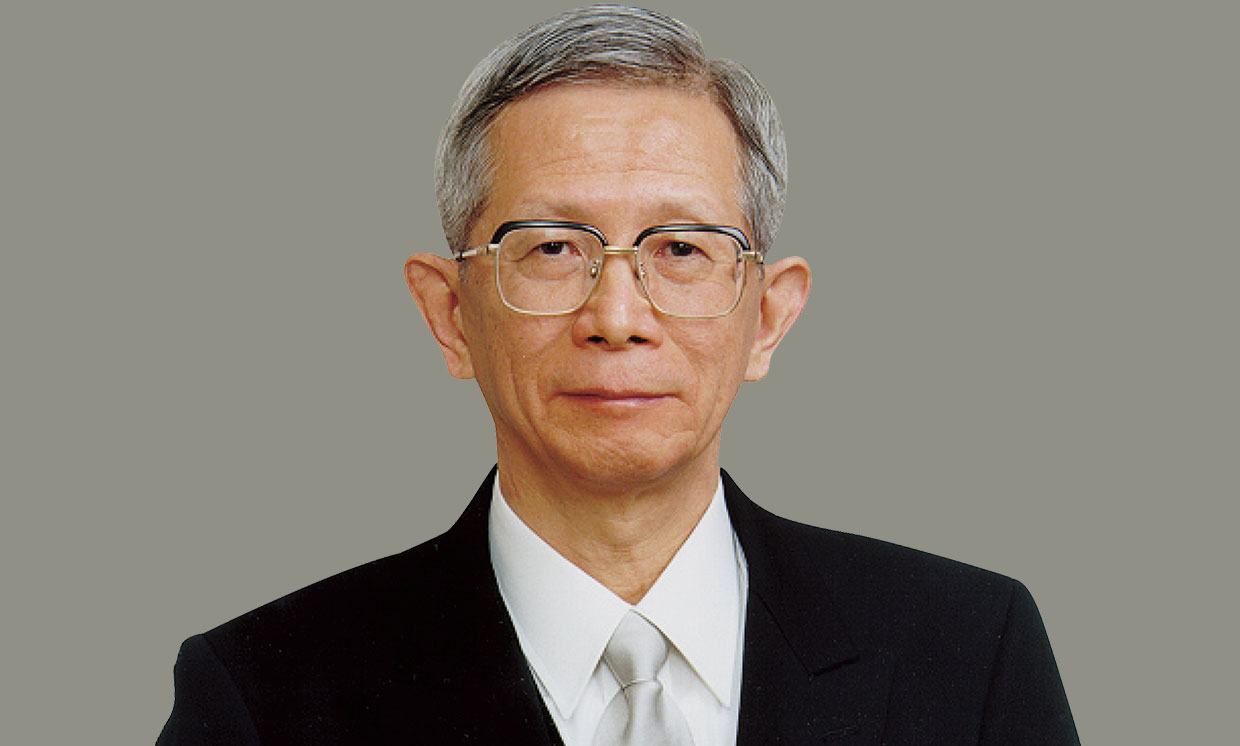
\includegraphics[width=0.5 \textwidth]{Aoyagi.jpg}	
	\caption{Dr. Takuo Aoyagi, inventor of the pulse oximeter.}
	\label{f1}       % Give a unique label
\end{figure}




\section {Figure With Caption} \label{Fig_Chap_2}

If the figure contains a source in the caption, then the source should only appear in the text but not in the table of content. \color{blue} Here is how you do it:\color{black} 


\begin{figure}[ht]
	\centering
	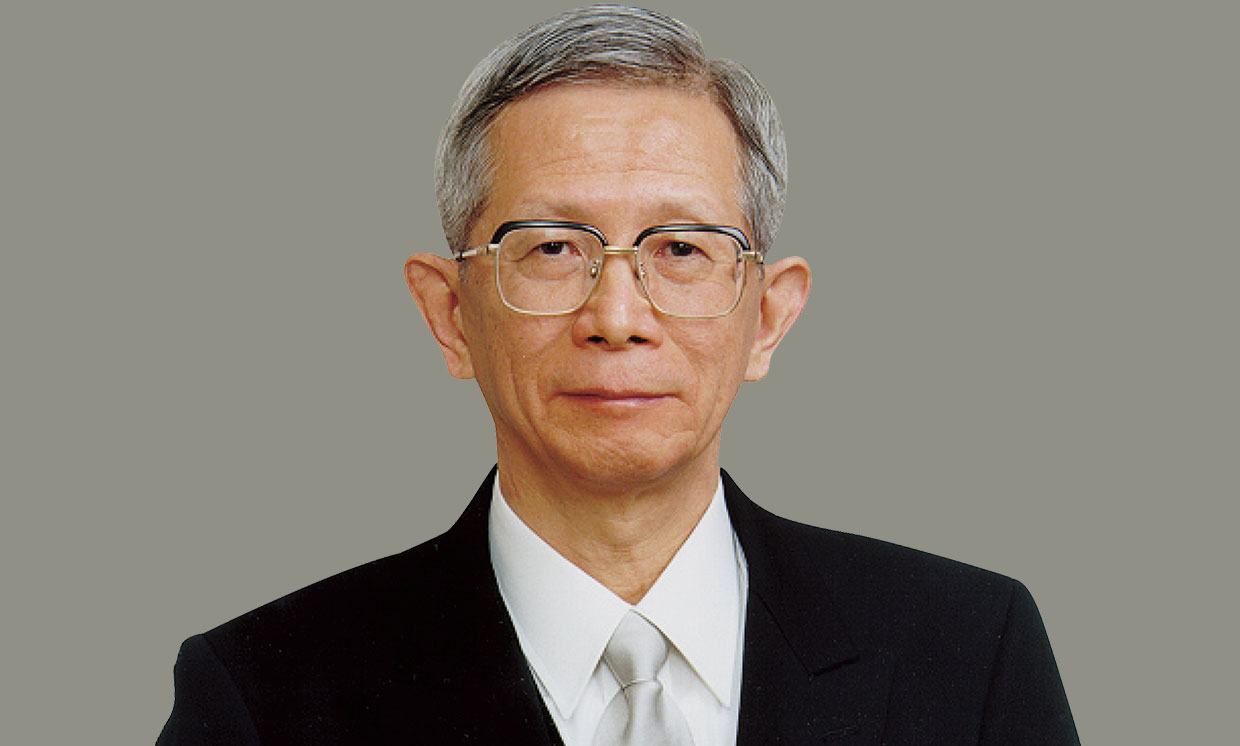
\includegraphics[width=0.5 \textwidth]{Aoyagi.jpg}	
	\caption[Dr. Takuo Aoyagi, inventor of the pulse oximeter.]{Dr. Takuo Aoyagi, inventor of the pulse oximeter. \\ \textit{\footnotesize Source: J. Goodrich, “Takuo Aoyagi, inventor of the pulse oximeter, dies at age 84,” IEEE Spectrum, 2022. [Online]. Available: https://spectrum.ieee.org/takuo-aoyagi-inventor-of- the-pulse-oximeter-dies-at-age-84. [Accessed: 20 February 2023]. }}
	\label{f2}       % Give a unique label
\end{figure}

\newpage

\section {Figure With Subplots} \label{Fig_Chap_3}

\begin{figure}[h!]
	
	\centering
	
	\begin{tabular}{c}	
		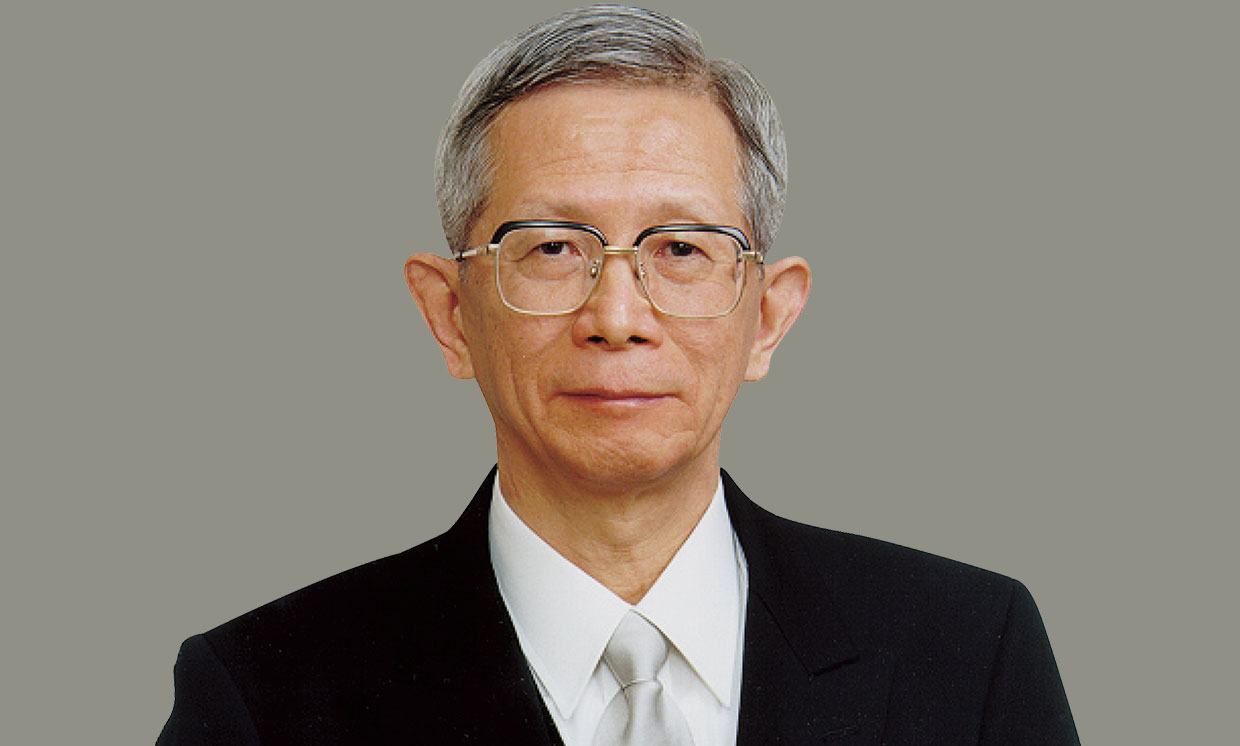
\includegraphics[width=0.5 \textwidth]{Aoyagi.jpg} \\
		(a) \\
		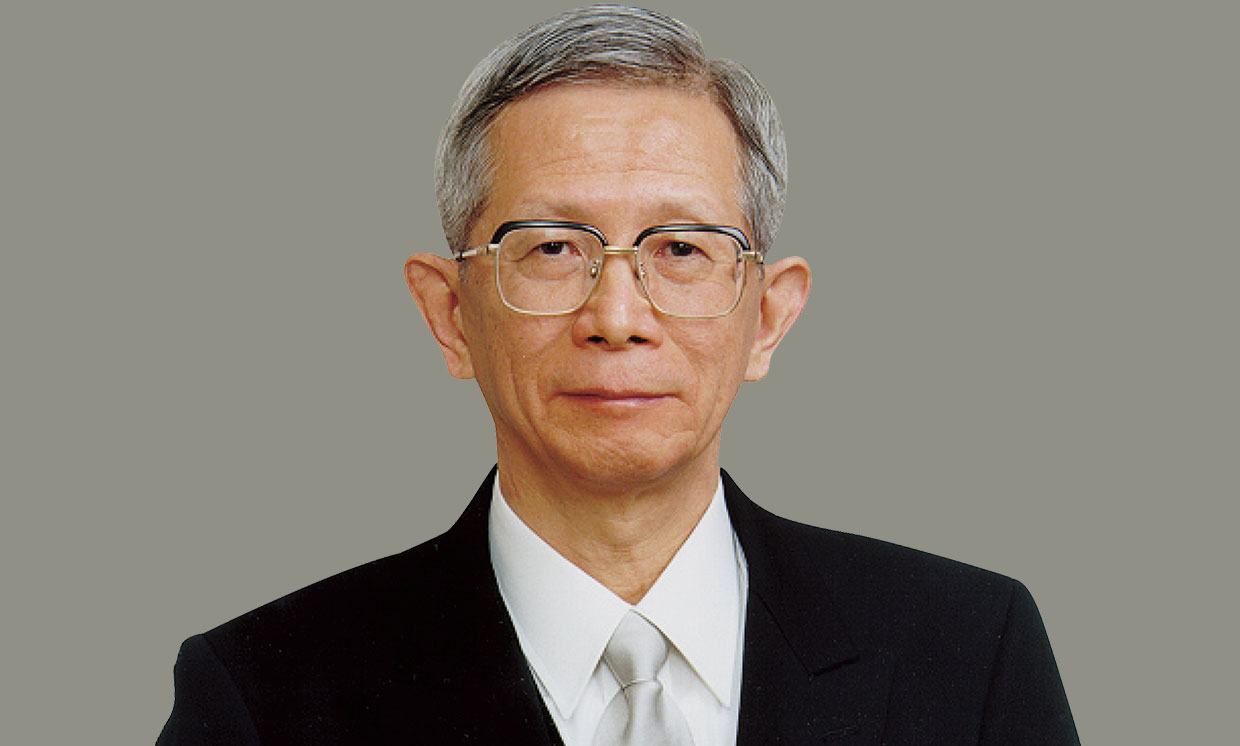
\includegraphics[width=0.5 \textwidth]{Aoyagi.jpg} \\
		(b)\\		
	\end{tabular}
	

	\caption{The subplots are atop of each other. (a) Something about subplot a. (b) Something about subplot b.}
	
	\label{f3}
\end{figure}




\begin{figure}[h!]
	
	
	\centering
	
	\begin{tabular}{cc}	
		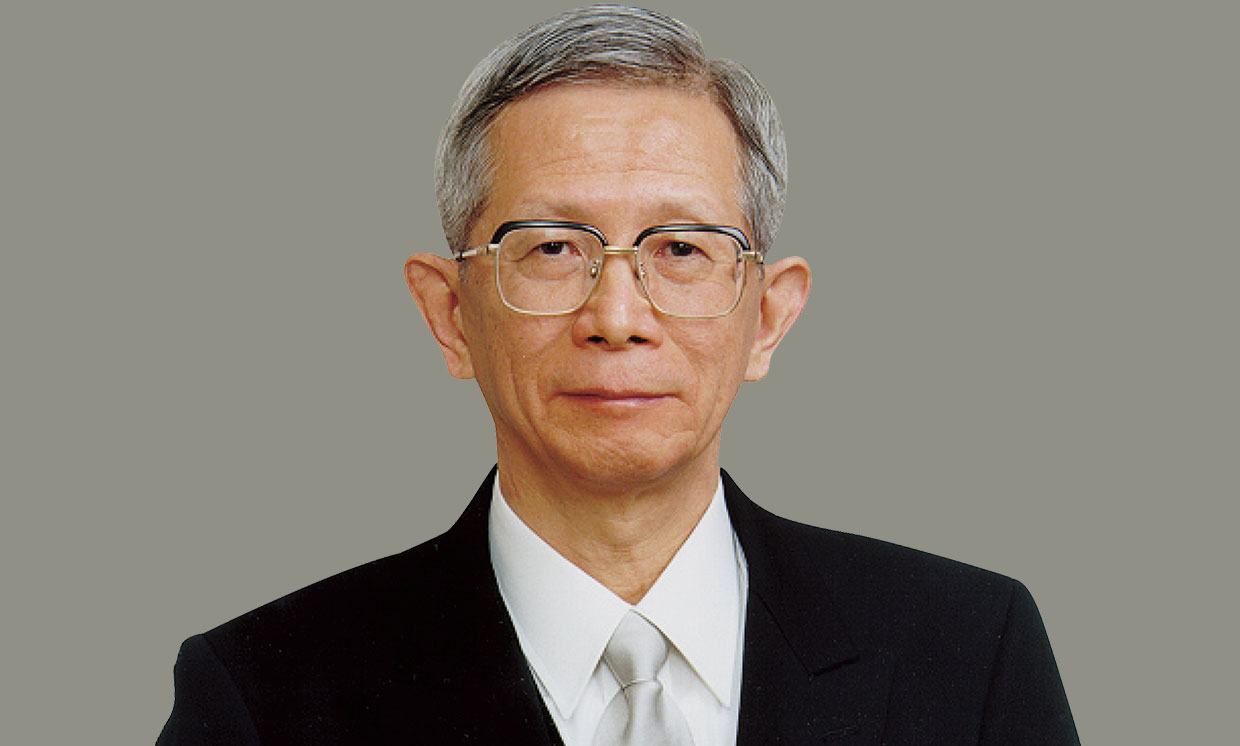
\includegraphics[width=0.35 \textwidth]{Aoyagi.jpg} & 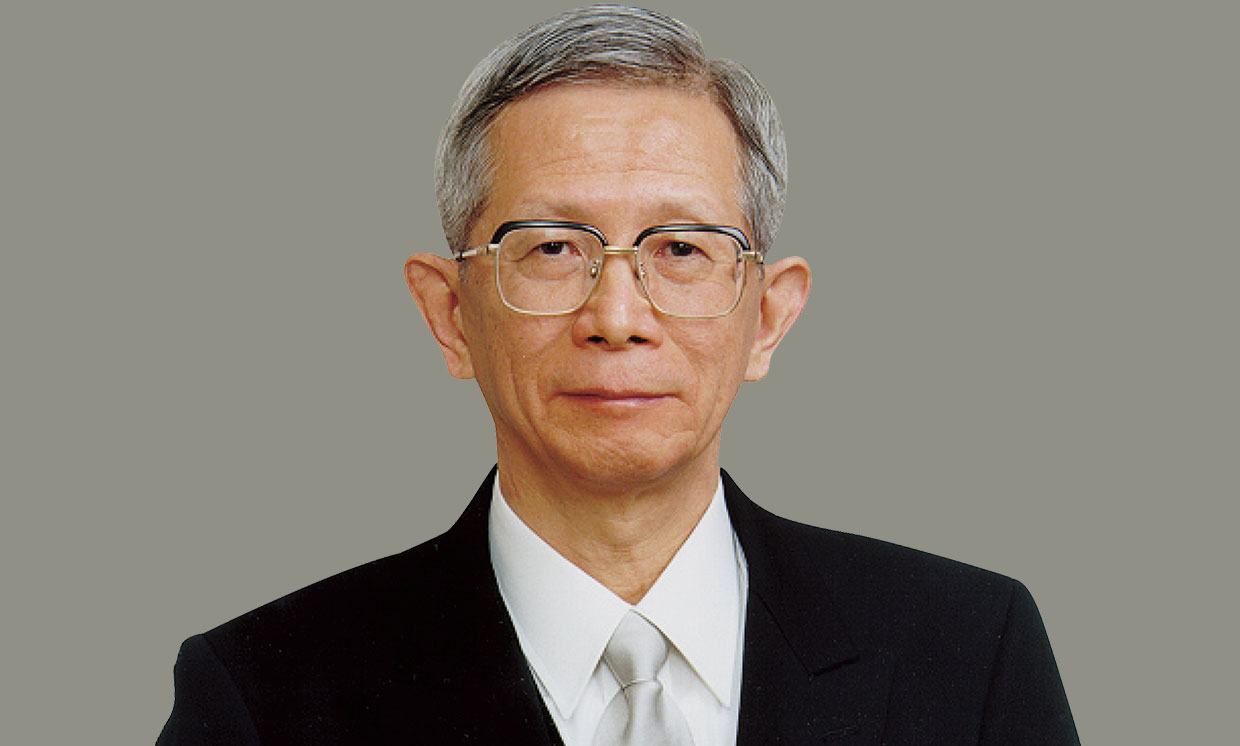
\includegraphics[width=0.35 \textwidth,angle=90]{Aoyagi.jpg}  \\
		(a)  & (b)\\		
	\end{tabular}
	
	
	\caption{The subplots are next to each other. (a) Something about subplot a. (b) Something about subplot b.}
	
	\label{f4}
\end{figure}


\section {Sideways Figure} \label{Fig_Chap_4} 

\begin{sidewaysfigure}
	\centerline{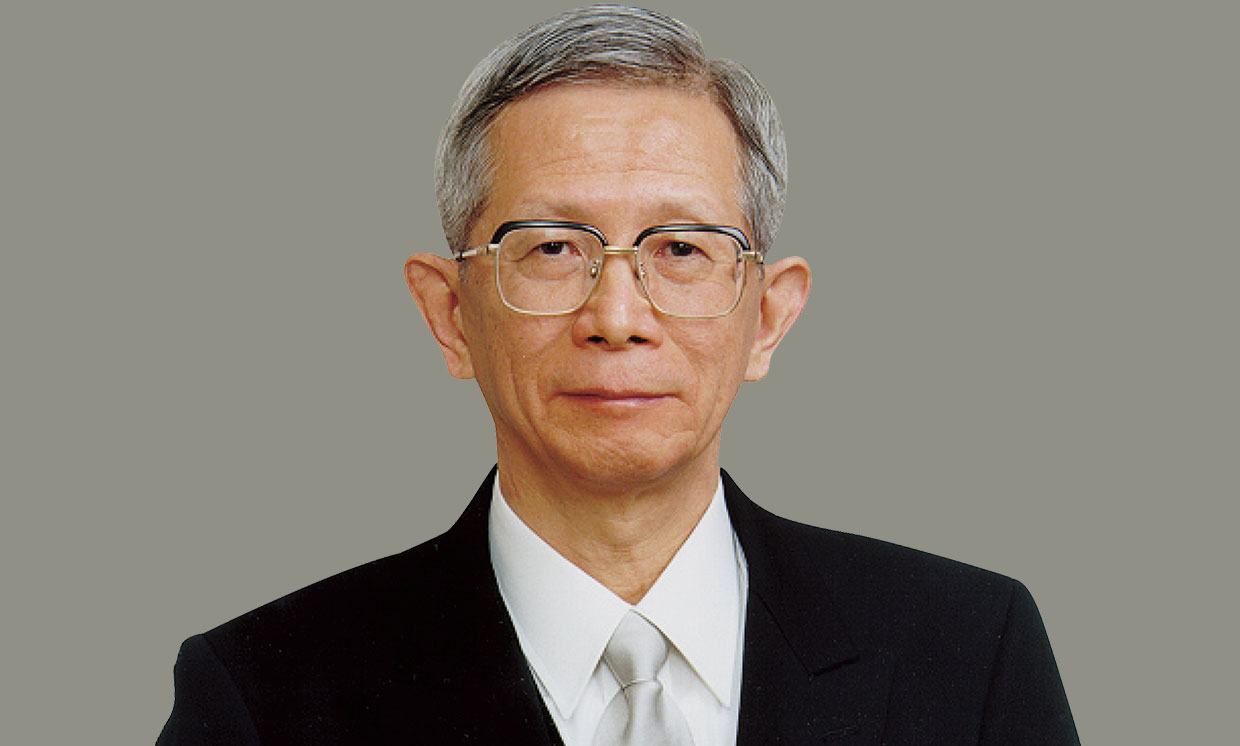
\includegraphics[width=120mm , angle = 0  ]{Aoyagi.jpg}}
	\caption{Sideways figure.}
	\label{f5}
\end{sidewaysfigure}




\chapter{Numbered Paragraphs and Footnotes}  \label{Chap3_ECG_HR_Tuned_Comb}

We can also create numbered paragraphs \vspace*{-7mm} 

\begin{enumerate} 
	 	\begin{singlespace}
	 \item First sentence First sentence First sentence First sentence First sentence First sentence First sentence First sentence First sentence. 
	 
	 \item Second sentence.
	 
	 \item Third sentence.
	 
  	\end{singlespace}
 \end{enumerate}

\color{blue} Note the spacing in the code.\\

\color{black} Or like this 
 
 
 \begin{itemize}
 	 	\begin{singlespace}
	 \item First sentence First sentence First sentence First sentence First sentence First sentence First sentence First sentence First sentence.  
	 
	 \item Second sentence.
	 
	 \item Third sentence.
	 
  	\end{singlespace}
\end{itemize}  


\color{blue} Numbered paragraphs must be single spaced with double space between consecutive paragraphs. The same goes for footnotes.\footnote{\color{blue} Write your footnote here. } \color{black}


This is how we can cite a random article using BibTeX \cite{Beethoven1800}.















%as required. Don't forget to give each section
%and subsection a unique label (see Sect.~\ref{sec:1}).
%\paragraph{Paragraph headings} Use paragraph headings as needed.




































 % comment out or remove if you don't need it
\chapter[Chapter about tables also chapter name is very lengthy it does not fit on one page]{Chapter about tables also chapter name is very \\ \vskip -3mm lengthy it does not fit on one page}\label{chap_tables} 


\color{blue} Below are some examples on how to generate tables with different formats. Tables can be also generated automatically using ``LaTex Table Editor'' available online.

\color{red}  NOTE: No ``.'' is needed at the end of the table title.

\color{black}
\section{Regular Tables}

\begin{table}[th]
	
	\begin{singlespace}
		\caption{Title Table Must Be All Capitalized}
		\label{CF_Eq_Tab}       % Give a unique label
		
		
		\renewcommand{\arraystretch}{1.5}
		\centering
		
		\begin{tabular}
			{|m{ 0.42 \textwidth} |m{ 0.51 \textwidth}|} \hline
			
			Item 1 & Description about Item 1. The description should be in single space.  \\
			\hline
			
			
		Item 2 & Description about Item 2. \\ 
			\hline
			
		\end{tabular}
	\end{singlespace}
	
\end{table}




\section{Special Table I}


\begin{table}[h]
	\begin{singlespace}
		\caption{Special Table One}

			
			\renewcommand{\arraystretch}{1.25}
			\centering
			
			\begin{tabular}{ |m{0.8cm} |m{1cm}  |m{2.2cm} |m{3cm} |m{4cm}|} 
				\cline{2-5} %\noalign{\smallskip} \noalign{\smallskip}
				\multicolumn{1}{c}{} \vline &   \textbf{X1}  & \textbf{X2} & \textbf{X2} & \textbf{X3} \\ 
				
				%\noalign{\smallskip} 
				\cline{1-5}
				
				\multirow{3}{*}{\rotatebox[origin=c]{90}{ \shortstack {\textbf{Text 1}  \\ \textbf{Text 2}}}}
				&$a_1$ & Blue &X &sensor data 1\\		
				\cline{2-5}
				&$a_2$ & Red  &Y &sensor data 2\\
				\cline{2-5}
				%\noalign{\smallskip} \noalign{\smallskip} \noalign{\smallskip}
				&$a_3$ & Orange &Z &sensor data 3 \\	
				
				%\noalign{\smallskip} \noalign{\smallskip} 
				\cline{1-5}
				
				
				
			\end{tabular}
		\end{singlespace}
		

	
\end{table}



\section{Special Table II}



\begin{table}[H]
	\begin{singlespace}
		%	\fontsize{7}{7}\selectfont 
		\caption{Special Table Two With Footnotes}
		\label{Tab_MAE}       % Give a unique label
		
		\renewcommand{\arraystretch}{1.2}	
		
		
		\centering
		\begin{tabular}{ |m{3.5cm}| m{3.2cm} |m{3.2cm} |m{3.2cm}|} 
			
			\cline{2-4} 
			\multicolumn{1}{c}{} \vline & \multicolumn{3}{c|} {\textbf{Metric Calculated for Methods}}  \\
			\cline{1-4} 
			{\textbf{Participants}} & {\textbf{Method 1}\color{blue}$^1$\color{black}}   & {\textbf{Method 2}\color{blue}$^2$\color{black}} & {\textbf{Method 3}\color{blue}$^3$\color{black}}\\ 			
			\cline{1-4} 	
			
			Participant 1 & 1 & 2 & 3 \\	 \cline{1-4}
			Participant 2 & 1 & \underline{2} & 3 \\	\cline{1-4} 
			Participant 3 & 1 & 2 & 3 \\	\cline{1-4}

		\end{tabular}
	\end{singlespace}
%	\vskip 4pt
	

	\begin{singlespace} 
		\vskip 4pt
		\footnotesize{\color{blue}$^{1}$ \color{black} You can put some information about method 1. We used a different color to make the superscript standout. The footnote should be single spaced. }
		\vskip 8pt
		\footnotesize{\color{blue}$^{2}$ \color{black} You can put some information about method 2. The footnote should be single spaced. }
		\vskip 8pt
		\footnotesize{\color{blue}$^{3}$ \color{black} You can put some information about method 3. The footnote should be single spaced. }
		
	\end{singlespace}
	
	
\end{table}







				  % comment out or remove if you don't need it

%\input{Preliminary_work}
%\input{Timeline}
%%%%%%%%%%%%%%%%%%%%%%%%%%%%%%%%%%%%%%%%%%%%%%%%%%%%%%
% REFERENCE LIST
%\bibliographystyle{elsarticle-num}

%\bibliographystyle{ieeetr}
\bibliography{library}



%%%%%%%%%%%%%%%%%%%%%%%%%%%%%%%%%%%%%%%%%%%%%%%%%%%%%%

\end{document}
